% Documentation:
%
% The UoK class file extends the standard report style to follow the Registry
% guidelines for laying out a thesis. It sets the margins, interline spacing,
% the page, figure and table numbering style, and disallows page breaks at
% hyphens. The class file consists of setting one and an half line spacing text
% with a 4cm left margin, at least a 2.5cm right margin, approximately 2cm top
% and bottom margin, on A4 paper.
% 
% The class the following options, in addition to those of the standard report
% class.
%     mini - Toggles the thesis in to mini-thesis mode. This adds "mini" to the
%            title and appends a nocite(*) at the end for an automatic output of
%            your complete bibliography.
%     draftmark - Puts a DRAFT' watermark on every page of the document along
%                 with the draft statement on the title page. Additionaly, it
%                 is used as a switch for the UoKExtentions package.
%     draft - Puts the entire document into draft mode. Applies all the effect
%             of draftmark above, but also propergates to other packages used.
%     copyright - Adds a copyright page between the title page and the preface.
%     nofig - Disables output of the list of figures in the preface.
%     notab - Disables output of the list of tables in the preface.
% All options passed to UoKthesis will be passed along to included packages:
%    natbib, draftwatermark, setspace, hyperref, lmodern
%
% The cover page and optional copyright page are implicitly added before the
% start of the preface section. Use the following commands to populate the 
% cover page/copyright page information:
%     \title{thesis title}
%     \author{author's name} 
%     \degree{Master of Science, Doctor of Philosophy, etc.} 
%     \subject{author's department}
%          - Computer Science if omitted 
%     \submitdate{month year in which submitted}
%          - dated by LaTeX if omitted 
%     \copyrightyear{year degree conferred (next year if submitted in Dec.)}
%          - assumes current year (or next year, in December) if omitted 
% 
% The preface environment allows for the use of sections that precede the main
% document; such as Abstract and  Acknowlegements. These sections should be
% defined using \section{Preface Section Title}. The contents page (and list of
% figures and tables if in use) will be automatically inserted at the end of the
% preface environment.
%
% The thesis style invokes the setspace package to set the commands:
%     \doublespace
%     \onehalfspace
%     \singlespace
% for spacing. By default one and an half spacing is used which resembles the
% UKC Typewriter requirement. Singlespace can be used for letterpress
% appearance. If you want to use true double space, for some reason, place the
% \doublespace command where you want to start using double spacing. Just call
% the appropriate spacing command at where you want to use them.
% 
% In the figure and table environments, single spacing is used. If you want to
% use any other size rather than one and an half spacing, then do:
% 	\renewcommand{\baselinestretch}{1.6} (or whatever you want instead of 1.6)
% This command won't take effect unless it comes before the \begin{document} or
% is triggered by a font change (after something like \small \normalsize).
%
% The example below shows the 12pt thesis style being used. This seems to give
% acceptable looking results, but it may be omitted to get 10pt. Alternatively,
% the 11pt option can be used.
%
% This version differs from old_ukcthesis.sty in the following ways:
% 1. Removed the doublespace package (now uses setspace).
% 2. Merged the phantom section for correct PDF links into the bibliography
%    generating function. 
% 3. Added thesis type options (mini, draft).
% 4. Kent Harvard is used for referencing and citation, this is supported by the
%    natbib package.
% 5. PsFig macro removed.
% 6. Now comes as two files, UoKthesis.cls, which defines purely stylistic layout,
%    and UoKextentions.sty, that provideds some additional functionality.

\documentclass[12pt]{UoKthesis}

%\renewcommand*\rmdefault{ptm}
%\renewcommand{\familydefault}{\rmdefault}
% Note: The UoKextentions package includes the xcolor package with the [usenames]
% options. If you need to add further options, these can be given to UoKextentions
% to be propogated through.
\usepackage{UoKextentions}
\usepackage{times}
%\usepackage{llncsdoc}
%\usepackage{verbatim}
\usepackage{url}
\usepackage{color}

\usepackage{amsmath}
\usepackage{relsize}
\usepackage[final]{listings}
\usepackage[T1]{fontenc}
%\usepackage[math]{times}
\usepackage{mathptmx}
\usepackage{graphicx}
\usepackage{wrapfig}
\usepackage[scaled=.90]{helvet}
\usepackage{courier}
\newcommand{\td}[1]{{\bf {\tt{#1}}}}
\newcommand{\comment}[1]{\textcolor{red}{\td{{#1}}}}
\usepackage{textcomp}
\usepackage{csquotes}
\lstset{
  frame=none,
  xleftmargin=2pt,
  stepnumber=1,
  numbers=left,
  numbersep=5pt,
  numberstyle=\ttfamily\tiny\color[gray]{0.3},
  belowcaptionskip=\bigskipamount,
  captionpos=b,
  escapeinside={*'}{'*},
  language=haskell,
  tabsize=2,
  emphstyle={\bf},
  commentstyle=\it,
  stringstyle=\mdseries\ttfamily,
  showspaces=false,
  keywordstyle=\bfseries\ttfamily,
  columns=flexible,
  upquote=true,
  showstringspaces=false,
  basicstyle=\small\ttfamily,
  breaklines=true,
  morecomment=[l]\%,
}

% Kent Harvard Bibliography Style. WIP
\bibliographystyle{kentHarvard}

% Provides nice linking in PDFs
\usepackage{hyperref}

% Only needed if you want to produce an index. Example is shown at the bottom of this document.
\usepackage{makeidx}

% Useful packages
% \usepackage{epstopdf} % Converts EPS files to PDF using ghostscript
% \usepackage{fnbreak}  % Warns you if you have split footnotes
% \usepackage{mathpazo} % Type­set­ math­e­mat­ics in the Palatino fam­ily of text fonts
% \usepackage{paralist} % Enumerate and itemize within paragraphs
% \usepackage{amsmath}  % AMS mathematical facilities
% \usepackage{rotating} % Rotating facilities for floats


\setcounter{secnumdepth}{3} % add more section types

%%%%% macros
\def\fixme#1{\fbox{\textbf{\textsc{Fixme}}\quad#1}}
\def\fixpic#1{\fbox{\textbf{\textsc{Picture}}\quad#1}}
\def\defnx#1#2{\emph{#1}\index{#2}}
\def\defn#1{\defnx{#1}{#1}}
\def\floatpic#1#2{%
\begin{wrapfigure}{r}{\dimexpr #1 / 2 \relax}
\includegraphics[width=\dimexpr #1 / 2 \relax]{#2}
\end{wrapfigure}}
\def\inlinepic#1#2{%
\begin{center}
\includegraphics[width=\dimexpr #1 / 2 \relax]{#2}
\end{center}}

%%%%% augment hyphenation
\hyphenation{wide-spread}

%%%%% document start
\begin{document}

\title{Data-Driven Refactorings for Haskell}
\author{Stephen Adams}
\subject{Computer Science}
\degree{PhD}

\begin{preface}
\section{Abstract}

Refactoring is the process of changing the internal structure of a program without changing its external behaviour. Refactoring increases code quality and reduces its technical debt. However, refactoring by hand is time consuming and error-prone. This makes automated refactoring tools very useful.

Agile software development allows for software to evolve slowly over time. This evolution changes how a program processes, abstracts over, and views its data. This evolution, though necessary, comes with the cost of technical debt. As technical debt increases changes to a code base become more difficult. Refactoring is one of the primary ways to  reduce technical debt. 

There exist refactorings that specifically help software to evolve its data model, however these refactorings are specific to the object-oriented programming paradigm. Haskell is a strongly typed, pure functional programming language. Haskell's rich type system allows for complex and powerful data models and abstractions. This thesis reports on work done to design and automate refactorings that help Haskell programmers develop these abstractions.

This work also discussed the current design and implementation of HaRe (the \textit{Ha}skell \textit{Re}factorer). HaRe now supports the Glasgow Haskell Compiler's implementation of the Haskell 2010 standard and its extensions. 

\section{Acknowledgements}
I would like to thank...
\end{preface}

\chapter{Introduction}\label{chp:intro}


\section{Functional Programming}
Functional programming is a programming paradigm that focuses on data values as described by expressions which are built from function applications and definitions~\citep{elementsOfFunc}.  Functions in this case are closely related to the idea of mathematical functions. Another key concept of a functional programming language is that functions are \textit{first class citizens}. This means that functions can be used like any other type of data, e.g. as arguments to other functions. 
  
\section{Haskell}
Haskell is a statically typed, lazily evaluated, pure functional language. Haskell is strongly and statically typed, and supports Hindley-Milner type inference~\citep{wikiIntro}. Type inference means that a Haskell programs do not need every type to be explicitly listed in the source code. Types will be~\textit{inferred} at compilation time so that every part of a Haskell program's type is known at that time. Haskell's type system also allows users to define their own types.

Lazy evaluation means that Haskell expressions are not evaluated when they are passes as a parameter, but rather when that value is used. For example in the Haskell function:
\clearpage
\begin{verbatim}
f x y = case x > 0 of
True -> x - 1
False -> x + 1
\end{verbatim}

The parameter y will never be evaluated.

Haskell is also a pure language. Purity is the idea that functions cannot perform actions in addition to returning values. These additional actions are known as side-effects. Haskell allows for traditionally side-effect causing operations (IO, state, etc.) through the use of monads. Monads contain any potentially side effect causing operations inside of them allowing the rest of the program to remain pure.

\section{Refactoring} 
Refactoring is the process of changing a program without changing its behaviour. This is done to improve its internal structure~\citep{fowler}. Behaviour preservation is what separates refactoring from other types of program manipulation. This idea of functionality preservation means that refactoring will not introduce new bugs or eliminate old ones. To prevent semantic changes after refactoring, many refactorings have non-trivial preconditions~\citep{refacTools}. 

Manual refactoring is tedious and error prone, and depends on high testing coverage to ensure that functionality is preserved~\citep{fowler}. This means that tools that can automatically perform refactorings and ensure that preconditions are met are highly desirable.

\subsection{Functional refactoring}

Refactoring a functional language has a few key differences from refactoring an imperative language. The higher-order nature functional languages means that any sub-expression of a function is a candidate for generalisation whereas in other languages the types of parameters and results is limited. The semantics of functional languages also allow for the complete checking of preconditions based on the static semantics of the language~\citep{refacTools}.

It is also not unusual for functional refactorings to be substantially different than their object-oriented (OO) counterparts. For example creating a case statement from a multi-equation function definition in a functional language versus inlining a virtual method as a case statement in an OO language require substantially different program manipulations~\citep{huiqingThesis}. Additionally there can be refactorings with no OO counterpart, monadification, for instance.  

\section{Contributions of this Research}

\comment{TODO}

\section{Justification and limitations of tooling}

A refactoring tool can only do so much the user needs to be "sufficiently smart" \comment{elaborate on this}

For tools to be successful they just have to bridge the gap between the original code to a version of the code that the programmer is willing to modify to what they want. Without the tool the transformation would be too risky or monotonous for the user to attempt alone.

  

\section{Thesis Outline}

\comment{TODO}


\chapter{Background: Refactoring Haskell in HaRe}
\label{hare}

\comment{
Chapter~\ref{hare} is where the development and implementation of HaRe will be discussed. The chapter with cover some of the history or HaRe and the briefly the technology that it was originally developed with. Next it will cover the design and implementation of HaRe currently and its dependencies (in particular ghc-exactprint). }

\td{
A brief outline of this chapter:

\begin{enumerate}
\item The original implementation of HaRe
\item The GHC API
\item Generic Programming (Scrap Your Boilerplate and Strafunski-StrategyLib)
\item GHC-ExactPrint
\item The Current version of HaRe
\end{enumerate}
}

Work on HaRe started in early 2003 at the University of Kent. HaRe was originally created by Huiqing Li, Claus Reinke, and Simon Thompson~\citep{refacWebsite}. This chapter begins with a brief discussion of the original implementation of HaRe. HaRe was originally implemented to support the Haskell 98 standard~\citep{huiqingThesis}. The Haskell ecosystem has evolved a great deal since then. Haskell 2010 is the current formal language standard but the Glasgow Haskell Compiler (GHC) has become the de facto Haskell standard~\citep{refacTools}. GHC supports the entire 2010 standard but also includes language extensions that do everything from changing the type system to adding new syntax features~\citep{langExts}.



\section{The original implementation of HaRe}

Implementing an automated refactoring system has several dependencies, a frontend for the language that you are targeting, a generic programming library, and a pretty printer. The language frontend is required for the refactorer to analyse and modify source code, the generic programming library assists in traversing the complex abstract syntax tree of a real world programming language, and the pretty printer outputs the modified AST in a form recognizable by the author of the original program. The original implementation of HaRe fulfilled these dependencies with two libraries, Programatica and Strafunski-StrategyLib. 

\subsection{Programatica and Strafunski}\label{prog&Strafunski}

Programatica was a project at the OGI School of Science and Engineering to build tool support for validating Haskell programs~\citep{programaticaTools}. The Programatica team open sourced their frontend so that other tools could also use it~\citep{refacWebsite}. The HaRe team chose to use Programatica over other available front ends (such as GHC's internal front end) because it was the simplest front end that supported the full Haskell 98 standard along with a number of its extensions~\citep{huiqingThesis}. Programatica's Haskell front end is broken up into multiple components including a lexer, a parser, an abstract syntax, a module system, a type checker, and a pretty printer. Programatica's frontend allows for HaRe to focus on refactoring only rather than having to build all of these components as well.

Programatica's abstract syntax contains 20 data types with 110 data constructors in total. Working with the syntax directly would introduce a large amount of "boilerplate" code into HaRe that would make maintenance and reusability of much more difficult~\citep{huiqingThesis}. Instead HaRe used Strafunski-StrategyLib, a combinator library for generic programming, to traverse the abstract syntax tree (AST) of the source code~\citep{strafunski}. 

Commonly transforming a program only modifies small sections of the source program's AST. Renaming a function, for example, will only need to modify the name used in the binding and places where that name is being used; all other sections of the AST remain unmodified. A commonly used operation in Strafunski takes a function that works on a particular data type (or types)\footnote{In the renaming example this could be code that checks if a variable is the one being renamed and replacing it with the new name.} and extends it to work on all types by leaving all other types unmodified. Strafunski also provides "strategies" that define how that extended function will be applied to the syntax tree~\citep{strafunski}\footnote{e.g. top-down or bottom-up}. The using Strafunski will be discussed in more detail in section~\ref{genProg}.

These two dependencies allowed the original implementation of HaRe to obtain the abstract syntax tree of source code to be refactored, traverse and transform that AST, and output the modified program. All these tasks are things that the current implementation of HaRe needs to do but the dependencies that it relies on have changed somewhat. The Haskell standard was updated in 2010~\citep{haskell2010} and GHC continues to expand the number of language extensions it supports. Unfortunately Programatica has not kept up with these changes and does not support anything beyond Haskell 98. At the same time GHC's own API has matured so that it can replace Programatica as HaRe's front end. HaRe now relies on this and a few other projects for its language frontend. For generic traversals "Scrap Your Boilerplate" has been added as a dependency though Strafunski-StrategyLib is still used~\citep{syb}.
 
\subsection{HaRe's original refactorings}\label{origRefactorings}

HaRe's original refactorings fall into three categories, structural, module, and data-oriented refactorings.

\subsubsection{Structural Refactorings}

Structural refactorings principally concern the name and scope of entities defined in a program~\citep{huiqingThesis}. These refactorings modify functions, and smaller sections of code. A traditional example of this is the renaming refactoring. 

Renaming is one of the most basic refactorings. The purpose of renaming is to change the name of a given identifier. A renaming refactoring could target a variable, function name, type, or any other piece of syntax that a programmer can name. This allows for the way in which you refer to your code to easily stay up to date with what your code actually does. 

Other examples of structural refactorings include deleting a definition, duplicating a function, and adding an argument~\citep{huiqingThesis}.

\subsubsection{Module Refactorings}

Module refactorings concern the imports and exports of an individual module, or the relocation of definitions between modules~\citep{huiqingThesis}. A simple refactoring in this category would be "clean an import list," which analyses a module's import list and removes redundant import declarations. Another example of a refactoring in this category would be the "move a definition" refactoring. As its name suggests, move a definition takes a definition from one module and moves it to another and fixes the imports and exports of any affected modules. For example if we were moving some function \texttt{foo} from module \texttt{A} to module \texttt{B} any external dependencies of \texttt{foo} need to be imported into \texttt{B} and if those dependencies are no longer used in \texttt{A} the import relevant statements should be removed. If \texttt{foo} is still being used in \texttt{A} then \texttt{A} needs to import \texttt{B} (if it does not already do so). Finally any other modules that currently depend on \texttt{foo} need to now import \texttt{B} (if it's not already imported) and remove the import of \texttt{A} (assuming none of \texttt{A}'s other definitions are used).

\subsubsection{Data Type Based Refactorings}

The third category of refactorings are those that are associated with data type definitions~\citep{huiqingThesis}. "Add field names" is a good example of a data-oriented refactoring.  The add field names refactoring will add field names to a data type. These names can then be used as selector functions that make extraction of a particular part of a type a simple function call. The new field names are generated by HaRe but can be renamed by the user~\citep{huiqingThesis}.

The adding of field names alone seems like an unusual 
\comment{Add description of concrete to abstract data type refactoring. Also use it to introduce composite refactoring. See: https://www.cs.kent.ac.uk/projects/refactor-fp/catalogue/ConcreteToAbstract.html and huiqings thesis}

These original refactorings were chosen to be basic yet still useful, and for their ability to give insight into the issues surrounding implementing an automated refactoring tool~\citep{huiqingThesis}. In addition to the refactorings that were implemented by HaRe's developers an API was exposed so that other developers could implement their own refactorings~\citep{hareApi}.


\subsection{The HaRe API}\label{hareApi}

Early in the development cycle of HaRe it was restructured to expose an API for implementing refactorings and general Haskell program transformations~\citep{hareApi}. The HaRe API contains a collection of functions for program analysis and transformation of Haskell 98 programs. These functions along with the functionality provided by Strafunski and Programatica form the basis for implementing basic refactorings~\citep{hareApi}.

The HaRe API exposes the full Programatica abstract syntax for Haskell 98 to the user but because of generic programming with Strafunski only the to be transformed parts of the AST have to be explicitly referenced in a refactoring~\citep{hareApi}. Another key feature of the API was to hide layout and comment preservation allowing the programmer to focus on program transformation instead. Each subtree in the AST is tagged with its absolute location in the source file. Any modifications to the AST will change the location of all elements that occur after the change. The API abstracts over this cascade of changes that follows even the simplest of changes. The HaRe API transformation functions modify the token stream and the AST simultaneously which keeps refactoring definitions free of this location bookkeeping ~\citep{hareApi}. 

The overall goal of the HaRe API is to help ensure the correctness of new refactorings by limiting the amount of code required that is not related to program transformation, and isolating common error sources~\citep{hareApi}. This design goal still guides the development of HaRe, and many of the functions that were provided in the original HaRe API have been updated to HaRe's latest implementation. 
 
\section{Underlying technologies}

As was mentioned in Section~\ref{prog&Strafunski}, HaRe's dependencies have changed somewhat in its current implementation. HaRe originally used Programatica as its front end, now the language front end is composed of several projects now, the GHC API, ghc-mod, and ghc-exactprint~\citep{ghcApi}, \citep{ghcMod}, and \citep{exactprint}. The following sections will describe these dependencies as well as Scrap Your Boilerplate~\citep{syb}, another generic programming library, and how HaRe currently uses them.

\section{The GHC API}

Rather than being a monolithic executable, the Glasgow Haskell Compiler (GHC) is composed of several smaller components that each correspond to a separate compiler stage. GHC's executable consists of a lightweight main function that ties together the smaller components~\citep{ghcDesign}. These components are exposed to users  and this is what constitutes the GHC API.

\subsection{Compiler stages of GHC}\label{ghcStages}

\begin{figure}[t]\label{compilerStages}
	\begin{center}
		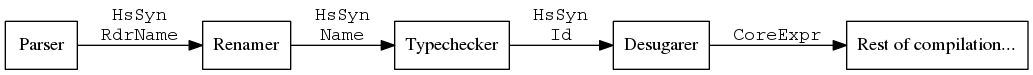
\includegraphics[scale=.4]{graphVis/Chapter2/compilerStgs.png}
	\end{center}
	\caption{GHC Compiler stages.}
\end{figure}

Some of the major components and the order that GHC uses them are shown in figure~\ref{compilerStages} which has been adapted from~\citep{ghcDesign}. This figure is not a complete list of all the components GHC uses just the parts that HaRe interacts with. The full diagram can be found in~\citep{ghcDesign}. The label after each compiler stage indicates the type of AST that is produced by that stage.

The top level datatype for all of the GHC abstract syntax is \texttt{HsSyn} ~\citep{ghcDesign}. \texttt{HsSyn} is parameterised by some identifier type; each compiler stage produces a different type of identifier with the additional information that stage produces. For example the typechecker takes in an AST parameterised by \texttt{Name} and returns an AST parameterised by \texttt{Id} which is a \texttt{Name} with additional type information.

\subsection{GHC's Name Types}\label{ghcNames}

There are five name types that GHC uses, they are:

\begin{itemize}
	\item \texttt{OccName} is the simplest type of name. It is just a wrapper around a \texttt{FastString} and an optional \texttt{NameSpace}. An \texttt{OccName} is contained in each of the other four identifier types.
	\item \texttt{RdrName} names are produced by GHC's parser. \texttt{RdrName}s aren't much more that an \texttt{OccName} with optional module information if the source name has been qualified. 
	\item \texttt{Name}s are produced by the renamer. A \texttt{Name} contains an \texttt{OccName} and a \texttt{Unique} that differentiates \texttt{Name}s that have the \texttt{OccName}. They have also had their scoping and binding resolved.
	\item \texttt{Id} \& \texttt{Var} are the identifiers produced by the typechecker.\footnote{\texttt{Id} is just a synonym for \texttt{Var}.} These identifiers both contain a \texttt{Name}, a \texttt{Unique}, and a \texttt{Type} or \texttt{Kind}. An \texttt{Id} has a definite type whereas a \texttt{Var} may contain type variables that only have a kind.   
\end{itemize}

These identifier types change throughout the compilation process but these names only parameterise the syntax tree, the shape of the tree itself stays the same through compilation. 

\subsection{GHC's syntax tree}
GHC's abstract syntax is currently made up of over 90 data types. Many of those types has multiple constructors, the expression data type \texttt{HsExpr} for example has over 40 constructors. This section will briefly introduce the structure of GHC's abstract syntax tree.

\subsubsection{Common syntax types}

The most common type in any given piece of GHC abstract syntax would be a \texttt{Located} as seen in listing~\ref{located}.

\begin{lstlisting}[caption={The \texttt{located} type.},label=located]

type Located e = GenLocated SrcSpan e

\end{lstlisting}

\texttt{Located} is used to tag syntax elements with their original position in a source file. The \texttt{SrcSpan} contains the filename that the span comes from and then the start and end columns and start and end lines that the span covers.\footnote{GHC has small optimisation where if a span exists entirely on a single line it only stores the single line number and the start and end column, instead of storing the same line number twice.} 

There are located versions of many of the AST types. For example, \texttt{HsExpr} is the type that represents expressions there is a related type \texttt{LHsExpr} that represents a located expression.

\begin{lstlisting}[caption={The located expression}]
type LHsExpr id = Located (HsExpr id)
\end{lstlisting}

The \texttt{HsExpr} type represents much of the Haskell language such as function application, lambdas, if and case statements. Pattern matching is handled by a \texttt{MatchGroup} type. Each \texttt{MatchGroup} contains a list of \texttt{Match}es and some typing information. Consider the following case statement

\begin{lstlisting}[caption={A case statement}, label=caseStmt]
case (x, y) of
	(Just i, Just j) -> Just (i+j)	
	(Just _, Nothing) -> x
	(Nothing, Just _) -> y
	(Nothing, Nothing) -> Nothing
\end{lstlisting}

This would be parsed into the \texttt{HsCase} constructor of \texttt{HsExpr}. This constructor is seen in listing~\ref{hscase}, the first constructor argument represents the expression that the patterns are matched against, (the tuple \texttt{(x,y)} in this case). The second argument to \texttt{HsCase} represents all four of the matches in the case statement. \texttt{MatchGroup}s are used to represent any code that associates some patterns with a right hand side expression. Function bindings, lambda expression, and case statements all use \texttt{MatchGroup}s. 

\begin{lstlisting}[caption={The \texttt{HsCase} constructor}, label=hscase]
HsCase (LHsExpr id) (MatchGroup id (LHsExpr id))	
\end{lstlisting}

In the case expression from listing~\ref{caseStmt} each of the four pattern matches is a \texttt{Match} in the expressions \texttt{MatchGroup}. Each \texttt{Match} associates a left hand side pattern with the appropriate right hand side expression.

\subsubsection{The syntax tree}
The previous section gave a brief overview of GHC's identifiers and its representation of expressions. This section describes the broader picture, the representation of whole Haskell programs.  

According to the GHC a Haskell program is simply a list of modules.\footnote{This is a very simple view and additional tools are needed to properly represent "projects" which is the context that most Haskell programs exist inside of. This is discussed further in section~\ref{hareInners}.} Inside of GHC each module is represented by an \texttt{HsModule}. This top level structure keeps track of everything that module imports, exports, and a list of all the declarations that the module defines. Declarations (of type \texttt{HsDecl}) are what represent everything that can be defined in Haskell. 

The \texttt{HsDecl} type is only used as a wrapper around other types. Bindings (of functions and/or values), instance, and type class declaration are differentiated by \texttt{HsDecl}'s constructors. 

\begin{lstlisting}[caption={A subset of \texttt{HsDecl constructors}}]
data HsDecl id =
	   TyClD (TyClDecl id)
	| InstD (InstDecl id)
	| ValD  (HsBind id)
\end{lstlisting}

\texttt{HsDecl} is only provides a single type that describes what sort of declaration it is. There is very little information stored at this level, the inner type is the "payload" of the declaration (e.g. \texttt{HsBind} or \texttt{TyClDecl}). These payload types are what store the type and expression level abstract syntax of Haskell that was described in the previous section.


\section{Generic programming}\label{genProg}
The need for a generic programming library, as previously discussed in section~\ref{prog&Strafunski}, remains the same when using the GHC API's AST as opposed to Programatica's. Currently HaRe still uses Strafunski-StrategyLib as well as another library, Scrap Your Boilerplate. Scrap Your Boilerplate (SYB) is a generic programming library developed by Ralf L{\"a}mmel and Simon Peyton-Jones~\citep{syb}.
\subsection{Generic Traversals}
The Stratego/XT library was one of first systems for programming tree transformations in a systematic way~\citep{stratego}. Stratego developed the idea of a transformation strategy. A strategy is the combination of a term rewriting function and a traversal function that describes how that rewriting function should be applied to a tree of terms. Stratego provides combinators that help construct term rewriting functions and tree traversal functions \citep{stratego}.

Stratego is an untyped transformation system and so was unsuitable for working with the statically typed Haskell.  
\subsection{Scrap Your Boilerplate}\label{syb}

	Suppose there was a simple expression language that contained integers, integer addition, assignment, and variables. This language is represented by the type defined below.
	
	\begin{lstlisting}[caption={A simple expression type.},label=expression]
type Name = String

data Expr =
     Value Int
   | Var Name
   | Add Expr Expr
   | Assign Name Expr
      deriving(Data,Typeable)
	\end{lstlisting}
	
	A function to rename a variable "x" to "a" is defined below:
	
	\begin{lstlisting}
renameXVar :: Expr -> Expr
renameXVar (Var "x") = Var "a"
renameXVar (Assign c e) = 
	| c == "x" = Assign "a" (renameXVar e)
	| otherwise = Assign c (renameXVar e)
renameXVar (Add e1 e2) = Add (renameXVar e1) (renameXVar e2)
renameXVar v = v
	\end{lstlisting}
	
	This is fairly straightforward and doesn't take much time to write. However, if subtraction was added to the definition of expression \texttt{renameXVar} would need to be updated as well to include a recursive call very similar to the addition case. These duplicated recursive calls are what is known as "boilerplate" code~\citep{syb}. Boilerplate code is highly repetitive, verbose, and difficult to debug and maintain.  In this small example having a few of these types of cases is not an issue. However, as the expression begins to approach the size of an actual programming language writing traversals like \texttt{renameXVar} become much more time-consuming and a nightmare to maintain. 
	
	The reduction of boilerplate code like this is the point of SYB. SYB allows us to rewrite \texttt{renameXVar} as:
	
	\begin{verbatim}
import Data.Generics	
	
rename :: Name -> Name
rename "x" = "a"
rename n = n

renameXVar :: Expr -> Expr
renameXVar = everywhere (mkT rename)
	\end{verbatim} 
	
	This example nicely illustrates the four key components of an SYB traversal~\citep{syb}.

	\begin{itemize}
		\item The function that performs the "interesting" part of the traversal
		\item A type extension for that function
		\item A generic traversal combinator
		\item The data type to be traversed must be an instance of the \texttt{Typeable} and \texttt{Data} classes (as explained below)
	\end{itemize}
	
	From the example mentioned previously the "interesting" part of this traversal is the rename function because this function contains the code that actually changes the name "x" to the name "a." The \texttt{mkT} function extends the type of the \texttt{rename} function to \texttt{Typeable~a = > a~ -> a}. 
	
	Type extension allows for the \texttt{rename} function to work over any members of the \texttt{Typeable} class rather than just \texttt{Name}s. The extended version of \texttt{rename} will work as expected when provided with an argument of type \texttt{Name}, and will act as the identity function if an argument of any other type is provided.
	
	The \texttt{everywhere} function is this traversal's generic combinator, \texttt{everywhere} applies a generic function to every node in the tree. Finally as you can see in the declaration of \texttt{Expr} derives both the Typeable and Data classes so it can be traversed by \texttt{everywhere}. A member of the Typeable class has defined a generic representation of itself and members of the Data class implement generic folding operations. Put together these two classes are what allow a data type to be generically traversed. 
	
\subsubsection{Types of Generic Algorithms}

SYB defines three types of generic algorithms, transformations, queries, and monadic transformations. The \texttt{rename} example from the previous section is an example of a transformation. Transformations preserve the type of the structure that is traversed. Queries, on the other hand, are "type unifying" algorithms. Queries are good for summarizing information contained in a data structure. You would use a query, for example, to traverse an expression and collect all of it's the bound variables. Using the same expression type (listing~\ref{expression}) from the previous section the following function extracts all bound variables from a given expression.

\begin{lstlisting}[caption={A generic function that collects all bound variables from an expression.}]
bVars :: Expr -> [Name]
bVars e = everything (++) ([] `mkQ` f) e
	where f (Assign nm _) = [nm]
          f _             = []
\end{lstlisting}

\texttt{everything}, as seen in the \texttt{bVars} function from the previous listing, is the generic query combinator that summarises all nodes, top down from left to right~\citep{sybDocs}. The first argument to \texttt{everything} is the function it uses to combine separate results from the query. In this case all the lists of names will be appended together. The "interesting" function \texttt{f} that actually returns a \texttt{Name} when one is being bound is extended via the \texttt{mkQ} function. \texttt{mkQ} will apply \texttt{f} when possible otherwise it will just return the empty list.

It is also useful a lot of the time to do transformations from within some monadic context. A simple example of this would be to rewrite the finding bound variables example from previously but instead the list of found results is stored as a piece of state.

\begin{lstlisting}[caption={Finding bound variables using the state monad}]
type TransformState = State [Name]

bVars :: Expr -> [Name]
bVars e = execState findVars []
  where findVars = everywhereM (mkM f) e
        f :: Expr -> TransformState Expr
        f e@(Assign n _ ) = do
          modify (\lst -> n:lst)
          return e
        f e = return e
\end{lstlisting}

A big advantage of monadic traversals is that both querying and transformations can happen in a single pass. The example in listing~\ref{renameVars} renames every \texttt{Name} in an expression by add \texttt{"\_old"} as a suffix and stores the original names in a list. 

\begin{lstlisting}[caption={Changing every found name and storing the old names in a list.},label=renameVars]
renameVars :: Expr -> TransformState Expr
renameVars e = everywhereM (mkM f) e
  where f :: Expr -> TransformState Expr
          f (Assign n e) = do
            modify (\lst -> n:lst)
            return (Assign (n++"_old") e)
          f (Var n) = return (Var (n++"_old"))
          f e = return e
\end{lstlisting}
 
This type of generic traversal is very common in HaRe because traversals often need to make use of a refactoring's stored state or run something from the GHC API which needs the features provided by a \texttt{GhcMonad} all while modifying the abstract syntax.   
	 
\section{ghc-exactprint}

After using generic programming to transform the parsed abstract syntax, HaRe needs to be able to print the modified code. A challenging part of building a refactoring tool is that a user wont want non refactored parts of their code to change at all. HaRe needs to preserve the user's comments and spacing from the source file.

Prior to GHC version 7.10.1 the location of certain keywords and punctuation (such as \texttt{do} and \texttt{let}) and user comments were lost after parsing. This made parsing and then printing an exact copy of a GHC Haskell file impossible. GHC's 7.10.1 release added annotations for the "lost" syntax elements that had previously not been represented in the parsed abstract syntax~\citep{apiAnns}. 

The parser produces a map that associates the keyword and the source span that the keyword can be found in with that keywords exact location. This approach was taken to avoid littering the existing AST with functionally meaningless keyword data~\citep{apiAnns}. 

Even with the position of every syntax element being recorded, printing a module after the AST has been modified is not easy. Many AST elements are "located" with a source span that indicates that element's exact position in the file. This means that any change to the AST will require updating the location of all the syntax elements that occur later in the line at least for single line changes and, in the case of changes that modify entire lines, every element after that change will need its location to be updated.

Ghc-exactprint simplifies this immensely by allowing us to position elements relative to their neighbours rather than absolutely~\citep{exactprint}. After parsing a source file HaRe takes the annotations GHC returns with the parsed abstract syntax and relativise them using ghc-exactprint. For each syntax element ghc-exactprint creates a new data type called an "\texttt{Annotation}" which contains an offset that indicates where this element should be positioned compared to the previous element. Take for example the following definition.

\begin{lstlisting} 
f a = (a+ 1 )
\end{lstlisting}

The absolute position of the plus sign is row one column nine (GHC's locations are one-based) but using ghc-exactprint we instead can think of the position of the plus sign using the offset \texttt{(0,0)} because there is no space between it and the previous element (the variable \texttt{a}). Using this system the number literal following the plus sign has an offset of (0,1) because of the single column of space before it. 

The \texttt{Annotation}s are stored in a map that is keyed based on the parsed location of a syntax element and the string representation of the AST constructor. In the previous example the right hand side of the definition is located at the source span (1,7)-(1,13) which stands for row one columns seven through thirteen and GHC represents this expression with the \texttt{HsPar} which is a constructor for the \texttt{HsExpr} type. The source span and the constructor together can be combined to retrieve the annotation data associated with this bit of the AST. This syntax tree has two elements associated with it, the opening and closing parenthesis. Each of these keywords is given its own offset, which in this case is (0,0) for the opening parenthesis\footnote{The offset in this case is (0,0) and not (0,1) as you might expect because the space between the equals sign and the opening parenthesis is represented in the offset for the entire right hand side expression.} and (0,1) for the closing parenthesis. We could obviously infer from the use of the \texttt{HsPar} constructor that this tree is wrapped in parenthesis however the users specific spacing would be lost without the annotations.

Comments are another element of a source file that prior to GHC 7.10.1 were "lost" after parsing. Using ghc-exactprint comments are stored in the annotations associated with the next piece of syntax. In the following code snippet the comment on line three is added to the annotations associated with the declaration of the function \texttt{f} along with a delta position that indicates the comment is a single line before this declaration starts.

\begin{lstlisting}
type Name = String

--a comment
f i = i + 1
\end{lstlisting}



\section{The current implementation of HaRe}

We have just discussed the major components that HaRe depends on. The ghc-api give us access to the internal representation of Haskell, the generic programming libraries Scrap Your Boilerplate and Strafunski-StrategyLib allows HaRe to more easily work with that internal representation, and ghc-exactprint is how HaRe preserves the source files spacing when writing the output file. From this foundation we can make HaRe focused on refactoring rather than solving these more generic problems. This section will discuss how HaRe is implemented, what its API provides, and some general conventions that it's refactorings use.

\subsection{HaRe's inner workings}\label{hareInners}

The GHC API work within the \texttt{GhcMonad} that provides the features GHC needs to compile a single Haskell source file such as IO, logging warning, exception handling, and keeping track of the compilation session~\citep{ghcApi}. In reality Haskell programs consist of more than just single source files without dependencies. Projects are organised using build tools such as Cabal or Stack~\citep{cabal,stack} that handle these issues for the programmer. HaRe needs to be aware of the context that these tools provide because refactorings may change multiple modules or modify modules that import modules from external dependencies. In HaRe's case ghc-mod provides a monadic context that handles these build environments and compiler setup~\citep{ghcMod}. Within ghc-mod's context HaRe keeps track of the state of the refactoring session.

\begin{lstlisting}[caption={HaRe's Monad \texttt{RefactGhc}},captionpos=b, label=refactghc] 
newtype RefactGhc a = RefactGhc
    { unRefactGhc :: GM.GhcModT (StateT RefactState IO) a}
\end{lstlisting}

Listing~\ref{refactghc} shows the definition of HaRe's monad that each refactoring runs in. \texttt{RefactState} is an ADT that keeps track of all the settings, abstract syntax, and filepath for refactoring a single file. It is possible to refactor client modules by setting the filepath in the \texttt{RefactState} to target another module. HaRe will then parse and typecheck that module's information into the state for transformation.

Even though there are three types of the AST, the annotations are part of the parsed AST ghc-exactprint works with the parsed AST only. Once a refactoring has finished it is expected that the parsed source and annotations will reflect all the changes that the refactoring has made. HaRe's state still contains all three of the syntax trees because the renamed and typed source are useful for the additional information they contain about the source file. 

\subsection{HaRe's API}

Modifying and reasoning about GHC's abstract syntax and maintaining the associated annotations is still a complex task even with help from HaRe's dependencies. HaRe defines its own API to help fill this gap between its dependencies and its refactorings. In addition to the obvious functions that are required for running a refactoring within the \texttt{RefactGhc} monad the API also includes helper functions that make working with the state easier. 

HaRe also defines a large collection of program analysis and transformation functions. For example, pulling the binding of a top level variable from a module's entire abstract syntax tree is a task that many refactorings have to do so this functionality is part of HaRe's API. There are also small program transformations that are not in and of themselves refactorings but common low level modifications that are useful to several refactorings, such as adding a new import declaration or making a function infix by wrapping it in back quotes (the \texttt{`} character).

Additionally there are several transformations that don't affect the abstract syntax as much as they change the annotations that format ghc-exactprint's output. Adding new lines before a syntax element doesn't change the meaning of a program but is important for a refactoring's output to be well formatted and easy to read. 

HaRe's dependencies help abstract away the low-level\footnote{Low level from the perspective of a refactoring at least.} details of a language back-end, build tools, and pretty printing. HaRe's API tries to close the gap still left between the dependencies and the refactorings themselves. In the next section we will take a look at how HaRe's refactorings are implemented.

\subsection{Implementing Refactorings in HaRe}

HaRe actually requires very few things from a refactoring implementation. As was mentioned previously in section~\ref{hareInners} everything must run inside of the \texttt{RefactGhc} monad who's state is where the abstract syntax of a target module is stored. A refactoring is also expected to return a list of  "\texttt{ApplyRefacResult}s" which contains an updated parsed AST and annotations along with the filepath the AST originated from; this updated AST is what HaRe writes out as the result of the refactoring\footnote{HaRe actually outputs to a temporary file. When refactoring "file.hs" HaRe produces "file.refactored.hs." This allows programmers to check the result of a refactoring before overwriting the existing module.}  


Beyond those two features refactorings are free to be implemented however the programmer chooses. However, certain conventions have been adopted within many of HaRe's refactorings. When describing a refactoring one would imagine that checking \textit{pre}conditions would be the first thing the implementation of that refactoring computes. A more efficient implementation checks preconditions throughout computation alongside the AST transformation. Merging precondition checking with transformation saves the refactoring from traversing parts of the AST multiple times, for example, the renaming refactoring checks for name conflicts while it descends the AST replacing the old name with the new one. Obviously this strategy only works for certain preconditions the only precondition for deleting a definition is that the target definition isn't used. The transformation only affects the syntax tree of the definition to be deleted so the implementation of the refactoring has to do a separate scan of the rest of the target module and any of its client modules to determine if the target definition is used or not. 

\chapter{Data-driven refactorings}

Some refactorings focus on rewriting the structure of a program (e.g. refactoring an \texttt{if} to \texttt{case} statement) a data-driven refactoring focuses on the types that a program works over and \textit{how} that program manipulates those types. Any changes that a data-driven refactoring makes to the structure of the program are \textit{driven} by the data types of that program rather than being the main motivation of performing the refactoring.

This chapter will begins in section~\ref{ooRefs} with a discussion of data-driven refactorings for imperative object-oriented languages. Imperative programs are written as a sequence of steps that modify an object to the desired output state. Types in an object-oriented also exist in a strict hierarchy. These two factors mean that object-oriented data-driven refactorings modify the hierarchy while leaving the structure of the code mostly intact. The rest of this chapter will describe data-driven refactorings for functional programs.

In comparison to the imperative way of constructing programs, functional programs tend to describe the relationship between the input and output data. Functional programming languages also tend to offer a much richer type system than object-oriented languages where data types are typically either objects or a set of non-user expandable primitive types. These two facts mean that the structure of a functional program can be determined by the types it works over to a much greater degree than in imperative languages. 

Section~\ref{introSyn} describes the introduce type synonym refactoring. This is the renaming of data-driven refactorings, neither the structure nor the type of the target program changes just how the program refers to the types it works over. Next, section~\ref{genMaybe} describes a generalisation refactoring. This thesis outlines two generalisations, one (described in section~\ref{genMaybe}) makes code of a specific type (\texttt{Maybe}) work over a type class (\texttt{MonadPlus} or \texttt{Monad}) instead. The other generalises code of one type class to use a class higher the hierarchy(covered in chapter~\ref{applicative}). Finally section~\ref{listToDlist} describes a refactoring that tranforms programs that work over lists to instead use an alternate implementation of lists. The refactoring method described in this chapter could be applied to refactor between types that can be projected onto another type.

\section{Object-Oriented Data Refactorings}\label{ooRefs}

The origins of refactoring are deeply rooted in the object-oriented world~(\cite{programRestructuring},~\cite{refactOOFrameworks}). Though it traces its origins to work on transforming Algol~\citep{recursiveTransformation}. The canonical catalogue of refactorings remains Martin Fowler's \emph{Refactoring: Improving the Design of Existing Code} ~\citep{fowler}. Fowler's catalogue of refactorings are all written in Java though he purposefully avoided using any features that were unique to Java, so that the refactorings could be applicable in many different programming languages.

As a functional programmer when going through this catalogue of refactorings there seem to be three types of refactorings.

\begin{itemize}
	\item Refactorings that are directly applicable in a functional language
	\item Refactorings that could be adapted for use in a functional language
	\item Refactorings not applicable to a functional language
\end{itemize}

That first type of refactorings' are structural refactorings and their usefulness to a functional program is easily understood. Refactorings like renaming or adding a parameter don't depend on object-oriented features existing in the target language.

The third type of refactorings are so dependent on features associated with object-oriented languages that they are impossible to implement or have no equivalent in a functional language. The "remove setting method" refactoring depends on the common OO pattern of each field of a class having "getter" and "setter" methods that retrieve or modify that field respectively. This pattern, on the other hand, is not as ubiquitous in functional languages because most do not support objects and immutability makes a "setter" function irrelevant. OCaml would be a notable exception to this rule: OCaml supports objects and allows the programmer to mark variables as mutable, and so getter and setter methods are possible.

\begin{figure}[t]
\begin{lstlisting}[language=caml, morekeywords={object,method}]
let mInt init_i = object
    val mutable i = init_i

    method get_i = i
    method set_i new_i =
      i <- new_i
  end
\end{lstlisting}
\caption{An OCaml object with getter and setter methods.}
\label{ocamlObj}
\end{figure}

The OCaml object from figure~\ref{ocamlObj} would be a valid target for this refactoring. However these methods are not as common as they are in imperative object-oriented languages with mutable data as the default, so a refactoring to remove a setter method is of limited value even for OCaml.

The second type of refactoring found in~\citep{fowler} is much more interesting to a functional programmer. The specifics of these refactorings are not directly applicable to functional programs but the underlying motivations are relevant to any programming paradigm. 

For example here is the motivation for the "Replace Data Value with Object" refactoring in~\citep[pg. 175]{fowler}:

\begin{displayquote}
Often in early stages of development you make decisions about representing simple facts as simple data items. As development proceeds you realize that those simple items aren't so simple anymore. A telephone number may be represented as a string for a while, but later you realize that the telephone needs special behavior for formatting, extracting the area code, and the like. For one or two items you may put methods in the owning object, but quickly the code smells of duplication and feature envy\footnote{Feature envy is when the methods of a class are more interesting in a different object than the one it is in.}. When the smell begins, turn the data value into an object.
\end{displayquote}

This refactoring extracts a field that was some primitive type into an object. The example from~\citep{fowler} works over an order class with a string that represents the customer that placed an order.

\begin{figure}[t]
\begin{lstlisting}[language = java,tabsize=4]
class Order {
	public Order (String customer) {
		_customer = customer;	
	}
	
	public String getCustomer() {
		return _customer;
	}
	
	public void setCustomer(String arg){
		_customer = arg;	
	}
	
	private String _customer;
}
\end{lstlisting}
\caption{The Order class}
\end{figure}

The refactoring creates a new customer class that has a string field with a getter method as seen in figure~\ref{custCls}. The customer class doesn't add any additional features but the extra layer of abstraction sets up the code base for further development. The customer object could have fields added that represent contact info or further demographic information without polluting the order class with order-irrelevant data.

\begin{figure}[t]
\begin{lstlisting}[language = java,tabsize=4]
class Order {
	public Order (String customer) {
		_customer = new Customer(customer);	
	}
	
	public String getCustomer() {
		return _customer.getName();
	}
	
	public void setCustomer(String arg){
		_customer = new Customer(arg);	
	}
	
	private Customer _customer;
}

class Customer {
	public Customer(String name){
		_name = name;
	}
	
	public String getName() {
		return _name;
	}
	
	private final String _name;
}
\end{lstlisting}
\caption{The result of the Replace Data Value with Object refactoring when applied to the customer field of the order class.}
\label{custCls}
\end{figure}

Functional programmers have to make similar data representation decisions as the object-oriented programmer. At the start of a project representing a customer just by their name could be reasonable. As the project develops this can become a serious limitation and a more robust abstraction is required. 

This section introduced how object-oriented refactorings help build up the data model over the lifetime of a project. In an object-oriented language the primary abstraction method is to introduce additional objects. These sorts of refactorings for a language with a rich type system like Haskell offer many more choices for evolving the data model of a system. An equivalent, but simpler refactoring, in the Haskell case would replace the string type synonym with the abstract data type in figure~\ref{custData}. The rest of this chapter will describe refactorings for Haskell that support data model evolution.  

\begin{figure}[t]
\begin{lstlisting}
data Customer = Customer {name :: String}
\end{lstlisting}
\caption{The algebraic data type for \texttt{Customer}.}
\label{custData}
\end{figure}
\section{Data-Driven Refactorings in Haskell}

Haskell offers a rich environment for data representation. The Haskell 2010 standard defines several types that are included in the prelude, including tuples, lists, characters, strings (which are just lists of characters), several types of numbers, and the function type. Additionally programmers can construct new types with algebraic and abstract data types or rename existing types with type synonyms. Type classes support overloading as well. The standard library of GHC comes with many type classes that can help produce powerful abstractions~\citep{typeclassopedia}. Contrast this with how most object-oriented type systems are either unified where every type is a subclass of some top level \texttt{Object} class (e.g. C\# or Ruby) or there are is a fixed set of predefined primitive types as well as the object hierarchy (e.g. C++ and Java's type systems). 

These two different approaches to type systems both have pros and cons which has sparked a vigorous (and quite possibly eternal) debate. The goal of this thesis is not to add to this debate, instead to build from a number of general principles that transcend the debate.

\begin{itemize}
	\item Data representation is a language independent problem that must be answered in every project.
	\item The way a project manages and represents its data is very likely to evolve over a project's lifetime and this is indeed desirable.
	\item Refactoring is a structured way to support this evolution.
		\item Refactorings for a language like Haskell need to take a different approach than those for object-oriented languages, particularly when refactorings are data-driven rather than ``structural.''  
	\item Data representation in a rich type system like Haskell's in some sense determines the structure of the program.
\end{itemize} 

\subsection{Introducing a Type Synonym}\label{introSyn}

Type synonyms in Haskell, as mentioned previously, are a way to name an existing type. A simple example can be seen in figure~\ref{fooSyn}. 

\begin{figure}[t]
\begin{lstlisting}
type Foo = (String, Int)

f :: Foo -> Foo
f x@(_, 0) = x
f (str, i) = (tail str, i-1) 
\end{lstlisting}
\label{fooSyn}
\caption{A simple type synonym.}
\end{figure}

Any place that where the \texttt{Foo} synonym is in scope the new name can be used to refer to any value of type \texttt{(String, Int)}. In fact "\texttt{Foo}s" and "\texttt{(String, Int)}s" are completely interchangeable. Introducing a synonym is a good way to quickly and simply name types to suggest their specific use in the current application.

Returning to the example from~\citep{fowler} of an order type that keeps track of the customer who placed the order used in section~\ref{ooRefs}, see figure~\ref{haskellOrder} for a Haskell implementation of this type and a function that counts how many orders a particular customer has placed in a list of orders.

\begin{figure}
\begin{lstlisting}
data Order = Order {customer :: String}

numberOfOrdersFor :: [Order] -> String -> Int
numberOfOrdersFor orders name = length (filter (\ord -> name == (customer ord)) orders)
\end{lstlisting}
\label{haskellOrder}
\caption{Using an algebraic data type for \texttt{order}.}
\end{figure}

The current representation of a customer as just a \texttt{String} is underdeveloped. Introducing a customer synonym is a simple step that sets up the code base for further development. The synonym will clearly mark which strings in the program stand for customers and which do not.

The introduce a type synonym refactoring works by taking a type and a valid synonym name (as per the Haskell 2010 standard~\citep{haskell2010}) and creates a new synonym. In this case the type is \texttt{String} and the synonym name should be something like "\texttt{Customer}." The only precondition of the refactoring is that the new synonym name cannot cause a name clash with any other variables in the same module and if the synonym is exported in any client modules that define something of the same name will need to qualify the import of the synonym. 

\begin{figure}[t]
\begin{lstlisting}
type Customer = String
\end{lstlisting}
\caption{The customer synonym}
\end{figure}

After this the next part of the refactoring involves replacing the appropriate uses of the type with the new synonym. This part of the refactoring is difficult to automate and needs to be interactive\footnote{This is not a feature of HaRe yet.}. There is no way to infer which instances of \texttt{String} (in the case of this example) should be replaced with the \texttt{Customer} synonym. The code from listing~\ref{haskellOrder} can have all of the string instances replaced by \texttt{Customer} because all the strings are being used to represent a customer. If there were a second function \texttt{printThankYou} which has type \texttt{String -> Order -> IO ()} which prints out a customized ``thank you'' message to the customer for their order. 

\begin{figure}[t]
\begin{lstlisting}
printThankYou :: String -> Order -> IO ()
printThankYou businessName order = do
	putStrLn ("Thank you " ++ (customer order) ++ " for your order.")
	putStrLn (businessName ++ " hopes to see you again soon!")
\end{lstlisting}
\caption{The \texttt{printThankYou} function}
\end{figure}

Though the first argument to \texttt{printThankYou} is a \texttt{String} it does not represent a customer therefore should not be replaced by the new synonym. The implicit meaning of the first argument hasn't been encoded in the type system so the programmer has to make a decision during the refactoring to make their intention for each instance of \texttt{String} clear. The final result of the refactoring can be seen in figure~\ref{orderRefact}. 

\begin{figure}[t]
\begin{lstlisting}
type Customer = String

data Order = Order {customer :: Customer}

numberOfOrdersFor :: [Order] -> Customer -> Int
numberOfOrdersFor orders name = length (filter (\ord -> name == (customer ord)) orders)

printThankYou :: String -> Order -> IO ()
printThankYou businessName order = do
	putStrLn ("Thank you " ++ (customer order) ++ " for your order.")
	putStrLn (businessName ++ " hopes to see you again soon!")
\end{lstlisting}
\label{orderRefact}
\caption{The program after adding a synonym for String.}
\end{figure}

 This transformation might seem like too small of a step. Wouldn't it be preferable to introduce a more powerful abstraction such as an algebraic data type? One of the principles of the Agile Manifesto is "simplicity" which is described as "maximizing the amount of work not done is essential"~\citep{agileManifesto}. The work not done in this case is the introduction of a more complex customer representation. This small step does clearly differentiate the strings that represent customers from other strings that represent other types of data.
 
Small refactorings are also a good practice for tool builders. Creating multiple small composable steps that can be used in multiple ways are much more flexible than large ``monolithic'' style refactorings.


\section{Generalising Maybe}\label{genMaybe}

A common type of refactoring is generalisation. A structural generalising refactoring would be extract a method or function. It takes expressions specific to a single function and generalises them so that they are applicable to multiple functions.

Data-driven generalisation is taking code written for a specific type and rewriting it to use a more general type. The newly generic code is applicable in more places and can help reduce code duplication. Fowler's Refactoring dedicates an entire chapter to generalisation, cataloguing refactorings like "extract subclass" and "extract interface"~\citep[pg. 319]{fowler}. 

Generalisations for object-oriented languages either move functionality up in a hierarchy (as in "push method up") or change the hierarchy by adding classes (e.g. "extract subclass"). Object-oriented languages have a single hierarchy since every object inherits from a root class typically just called \texttt{Object}. Functional languages don't have this single unified hierarchy, but smaller hierarchies do exist because type classes can inherit from one another. 

This section describes a refactoring that rewrites programs of type \texttt{Maybe a} to use the \texttt{MonadPlus} type class or, if possible, the \texttt{Monad} type class. 

\begin{figure}[t]
\begin{lstlisting}
data Maybe a = Nothing
                 | Just a
                 
instance MonadPlus Maybe where
   mzero = Nothing
   Nothing `mplus` r = r
   l          `mplus` _ = l
                 
class Monad m => MonadPlus m where
   mzero :: m a
   mplus :: m a -> m a -> m a
\end{lstlisting}
\caption{The \texttt{Maybe} data type definition and \texttt{MonadPlus} instance declaration, and the \texttt{MonadPlus} class definition.}
\label{maybeMonadPlus}
\end{figure}
 
Figure~\ref{maybeMonadPlus} contains the class declaration for \texttt{MonadPlus} the \texttt{Maybe} instance of that class. The \texttt{Maybe} type represents a computation that may return a value wrapped in the \texttt{Just} constructor or may fail (represented by the \texttt{Nothing} constructor). The \texttt{MonadPlus} class is a typeclass for monads that also have a monoidal structure~\footnote{A monoid is a semigroup whose associative binary operation has an identity element.}. 

The \texttt{MonadPlus} class helps generalise monads that contain some concept of failure and choice. The \texttt{mzero} value represents a failed computation and \texttt{mplus} represents a way of making a "choice" between two computations that may or may not have failed~\citep{typeclassopedia}. 

\begin{figure}
\begin{lstlisting}
class Applicative m => Monad m where
	return :: a -> m a
    (>>=)  :: forall a b. m a -> (a -> m b) -> m b
    
instance Monad Maybe where
	return = Just
	
	(Just a) >>= f = f a
	Nothing  >>= _ = Nothing
\end{lstlisting}
\caption{\texttt{Maybe}'s monad instance definition}
\label{maybeMonad}
\end{figure}

\subsection{Refactoring Maybe to Monad}\label{genMonad}

This refactoring replaces \texttt{Maybe}-specific code with the more general \texttt{Monad} and \texttt{MonadPlus} operations. This is done by recognizing when \texttt{Maybe}-specific code is structured in the same way as the more general operations. Figure~\ref{mmp1} contains a simple example of this.  

\begin{figure}[t]
\begin{lstlisting}
inc :: Maybe Int -> Maybe Int
inc Nothing = Nothing
inc (Just i) = (Just (i + 1))
\end{lstlisting}
\caption{\texttt{inc}}
\label{mmp1}
\end{figure}

The function \texttt{inc} can be rewritten to use the monadic operations bind (\texttt{>>=}) and \texttt{return} instead, this is because the definition of \texttt{inc} matches the definition of bind in the instance declaration of \texttt{Maybe} as a monad. Figure~\ref{incRewrite} has another version \texttt{inc} in which that relationship is clearer.

\begin{figure}[t]
\begin{lstlisting}
inc :: Maybe Int -> Maybe Int
inc x = new_inc x f

new_inc :: Maybe Int -> (Int -> Maybe Int) -> Maybe Int
Nothing `new_inc` _ = Nothing
(Just i) `new_inc` f = f i

f i = Just (i + 1)
\end{lstlisting}
\caption{\texttt{inc} rewritten to look more like bind}
\label{incRewrite}
\end{figure}

The new version of \texttt{inc} has been written using infix notation, to more closely match \texttt{Maybe}'s definition of bind. Also like \texttt{Maybe}'s bind when \texttt{inc}'s first argument is \texttt{Nothing} it just returns \texttt{Nothing}. Finally the right hand side of \texttt{inc}'s second case was lifted into a separate function and is passed to the new \texttt{inc} as an argument, just like \texttt{bind}.

In practice the refactoring will, by default, create an anonymous function from the right hand side of the \texttt{Just} case with calls to \texttt{Just} and \texttt{Nothing} replaced with \texttt{return} and \texttt{mzero} respectively. The final refactored version of \texttt{inc} is in figure~\ref{mmp1Ref} 

\begin{figure}[t]
\begin{lstlisting}
inc :: (Monad m) => m Int -> m Int
inc mi = mi >>= (\i -> (return (i+1)))
\end{lstlisting}
\caption{Final output from generalising \texttt{inc}}
\label{mmp1Ref}
\end{figure}

It is worth saying that if the right hand side of the \texttt{Just} case from the original implementation of \texttt{inc} contained calls to \texttt{Nothing} then this function could not be generalised to \texttt{Monad}. Instead, the anonymous function would replace the occurrences of \texttt{Nothing} with \texttt{mzero} instead.  
 
\subsection{Refactoring Maybe to MonadPlus} 

The first example could be rewritten using functionality provided only by the \texttt{Monad} type class. Obviously this isn't always the case. An example of a function that cannot be completely generalised to \texttt{Monad} is in listing~\ref{mmp2}.

\begin{figure}[t]
\begin{lstlisting}
showNat :: Int -> Maybe String
showNat i =
  if (i <= 0)
    then (Just (show i))
    else Nothing
\end{lstlisting}
\caption{\texttt{showNat}}
\label{mmp2}
\end{figure}

The function \texttt{showNat} takes in a pure value and returns a \texttt{Maybe}, instead of taking in a \texttt{Maybe} and returning another \texttt{Maybe} as in the previous example. The more general version of \texttt{showNat} needs to be able to express the idea of failure that \texttt{MonadPlus} encodes with the \texttt{mzero} operation. 

\begin{figure}[t]
\begin{lstlisting}
showNat :: (MonadPlus m) => Int -> m String
showNat i =
  if (i <= 0)
    then (return (show i))
    else mzero
\end{lstlisting}
\caption{\texttt{showNat} refactored}
\label{mmp2Ref}
\end{figure} 
 
Figure~\ref{mmp2Ref} shows the refactored version of \texttt{showNat}. In this case the refactoring can simply replace the \texttt{Maybe}-specific calls with more general ones. This is very similar to the way that the expression that made up the anonymous function from listing~\ref{mmp1Ref} was constructed by changing calls to \texttt{Just} to \texttt{return} and calls to \texttt{Nothing} to \texttt{mzero}. 

Due to the \texttt{return} operator of \texttt{Monad} being equivalent to \texttt{Just} and \texttt{mzero}being supplied by \texttt{MonadPlus}, both of \texttt{Maybe}'s constructors can be replaced with a more general operation. Between these two type classes all of the functionality of \texttt{Maybe} can be replaced in functions that build \texttt{Maybe}s. However if a function deconstructs a \texttt{Maybe} type through pattern matching it may not be generalisable. Consider the function \texttt{printResult} in figure~\ref{printRes}.

\begin{figure}[t]
\begin{lstlisting}
printResult :: (Show a) => Maybe a -> IO ()
printResult m =
  case m of
     Nothing -> putStrLn "Something went wrong"
     (Just i) -> putStrLn $ "The result is: " ++ (show i)
\end{lstlisting}
\caption{\texttt{printResult}}
\label{printRes}
\end{figure}

\texttt{printResult} uses \texttt{Maybe}'s constructors for pattern matching rather than in expressions; there is no generic pattern match for \texttt{Just}. Refactoring \texttt{printResult} will require the programmer to provide a way to convert its argument to \texttt{Maybe}.

\begin{figure}[t]
\begin{lstlisting}
printResult :: (Show a, MonadPlus m) => (m a -> Maybe a) -> m a -> IO ()
printResult f = printResult_old . f
   where
	printResult_old :: Maybe a -> IO ()
   	printResult_old m =
   	  case m of
  	  Nothing -> putStrLn "Something went wrong"
  	  (Just i) -> putStrLn $ "The result is: " ++ (show i)
\end{lstlisting}
\caption{Refactored \texttt{printResult}}
 \label{printRef}
\end{figure}
 
Figure~\ref{printRef} show the finished refactoring of \texttt{printResult}. The original definition of \texttt{printResult} is renamed and moved into a local definition. The new \texttt{printResult} function now takes in an additional parameter, an "abstraction function." The abstraction function abstracts the new type \texttt{m a} back to the old \texttt{Maybe a}. The inverse of the abstraction function is the projection function\footnote{In this specific case the projection function is of type: \texttt{Maybe a -> m a}}. These types of functions are used more in the next section (\ref{listToDlist}).

When passed the abstraction function \texttt{printResult} just converts the now genericly typed argument to \texttt{Maybe a} and then calls the original function definition.

In general this refactoring case doesn't do much. This is because its difficult to ``consume'' a more general type due to argument types being contravariant under the function type constructor.
 
\section{``Lists to Hughes Lists'' Refactoring}\label{listToDlist}

The previous section discussed a refactoring that is most useful in the early stages of development when the details of data representation are in their infancy. As a project develops more and more decisions must be made about how data is represented and processed. Mid-development it may become necessary to change which data structures the program uses in order to facilitate adding additional features or for performance reasons.

This section will cover a refactoring for automatically replacing a type by "projecting" that type into another. The two types (the original and the new type) don't necessarily to have a formal syntactic relationship from the compiler's point of view (e.g. both implement the same type class) but instead have an ad-hoc, semantic similarity. 

\subsection{Hughes Lists}

Appending two lists into a single list is a fundamental operation over lists. The standard implementation of append is seen on line one in figure~\ref{append}.\footnote{The \texttt{(++)} operator is the infix definition of append.} 

\begin{figure}[t]
\begin{lstlisting}
(++) :: [a] -> [a] -> [a]
[]  ++ ys = ys
(x:xs) ++ ys = x:(xs ++ ys)
\end{lstlisting}
\caption{The standard definition of append}
\label{append}
\end{figure}

If the first argument to append is the empty list then append can just return the second argument. In the other case append traverses the first list popping off the head of the first list and recursively appending the tail of the first list and the second argument. The performance of append is proportional to the length of its first argument. This has the unfortunate side effect that if a program builds of a list by repeatedly appending  to the end of a list the program will spend significant amounts of time traversing the beginning of the list over and over. In total the performance of this function ends up being $O(n^2)$ where $n$ is the length of the final list.

An example of a function that exhibits this behaviour is \texttt{countdown}, which is defined in figure~\ref{countdown}. \texttt{countdown} constructs a string that lists the numbers starting at the argument \texttt{i} down to zero. During each recursive call the previously computed result is traversed but this parameter gets larger each time which is what causes the $O(n^2)$ performance.

\begin{figure}[t]
\begin{lstlisting}
countdown :: Int -> String
countdown i = f i ""
  where f 0 s = s ++ "0"
          f i s = let newS = s ++ (show i) ++ ", " in
          f (i-1) newS
\end{lstlisting}
\caption{The countdown function runs in $O(n^2)$ time.}
\label{countdown}
\end{figure}

The poor performance of \texttt{countdown} quickly becomes noticable with \texttt{countdown 10000} taking around six seconds to run.\footnote{On an Intel i5 4690k processor with 16 GB of RAM}

Fortunately there is an alternative representative of lists that allows $O(n)$ time for such nested appends. This alternative representation was first described by John Hughes in~\citep{hughesList} (hence their name), they are also known as difference lists~\citep{realWorldHaskell}; difference lists is the name that they are provided by in Hackage~\citep{dlist}. In Hughes lists elements are stored as partial applications of the append function, these partial applications can then be composed together using function composition (the \texttt{(.)} operator in Haskell) to append the two lists together. 

Difference lists store the values \texttt{[1,2,3]} as \texttt{([1,2,3] ++)} which is of type \texttt{Num a => [a] -> [a]}. Appending \texttt{[4,5,6]} to \texttt{([1,2,3] ++)} first involves converting it to a difference lists (\texttt{([4,5,6] ++)} in this case) then these two difference lists can be appended with function composition which results in \texttt{([1,2,3] ++) . ([4,5,6] ++)}. 

\begin{figure}[t]
\begin{lstlisting}
> let lst = ([1,2,3] ++) . ([4,5,6] ++)
> :t lst
lst :: Num a => [a] -> [a]
> lst []
[1,2,3,4,5,6]
\end{lstlisting}
\caption{Building and deconstructing difference lists.}
\label{ghciDList}
\end{figure}

As seen in figure~\ref{ghciDList}, once it comes time to retrieve the normal list the difference list is applied to an empty list. Function composition is evaluated from right to left so this keeps the left operand of \texttt{(++)} small. Internally difference lists are just a wrapper around a function from lists to lists. Figure~\ref{dlistDef} shows the definition of the \texttt{DList} new type which contains the partial application. The \texttt{unDL} function simply removes the \texttt{DL} constructor. 

\begin{figure}[t]
\begin{lstlisting}
newtype DList a = DL {
   unDL :: [a] -> [a]
}

fromList :: [a] -> DList a
fromList xs = DL (xs ++)

toList :: DList a -> [a]
toList (DL xs) = xs []

append :: DList a -> DList a -> DList a
append xs ys = DL (unDL xs . unDL ys)
\end{lstlisting}
\caption{The definition of \texttt{DList} taken from~\citep{realWorldHaskell}}
\label{dlistDef}
\end{figure}

While difference lists support fast appends there is no such thing as a free lunch, speed ups for certain functions are paid for by slowdowns in other places. Getting the head and tail of a normal list are both constant time operations but become linear time for difference lists because the difference lists will have to be converted back to normal lists. 


\subsection{Refactoring lists to Hughes lists}

For functional programmers, lists are a very familiar and versatile data structure. However, if an application requires repeated appends as described at the start of this section their performance becomes an issue. Difference lists provide a similar interface to lists but without this troublesome behaviour. This section will describe a refactoring to convert programs written using normal lists to use difference lists instead. 

\subsubsection{Embeddable Types} 
This refactoring takes the view that a type consists of some structure and a set of functions that operate on that structure. 

This refactoring requires that a source type is ``reversibly embeddable'' into the target type. If the source type is some type $A$ and the target type is some type $B$ then for $A$ to be reversibly embeddable in $B$ two functions must exist. The projection function $proj :: A \rightarrow B$ and the abstraction function $abs :: B \rightarrow A$. The property in equation~\ref{eq1} must hold for $A$ to be embeddable in $B$. However, the property in equation~\ref{eq2} does not necessarily hold.   

\begin{figure}[t]
\begin{equation}\label{eq1}
abs . proj = id
\end{equation}

\begin{equation}\label{eq2}
proj . abs \neq id
\end{equation}
\end{figure}

Intuitively this means that it needs to be possible to retrieve the $A$ type from a $B$ exactly as it was when it was projected into the new type. The reverse does not need to be true because any values of type $B$ were introduced by the refactoring so any information lost converting a $B$ back into an $A$ wasn't in the original program and so does not need to be preserved to preserve behaviour.

In the "list to Hughes list" case the projection function is \texttt{fromList} (because it embeds lists into the new type \texttt{DList}) and the abstraction function is \texttt{toList}. How to define the set of pairs is an interesting problem with multiple solutions. The \texttt{Data.DList} module exports the following functions~\citep{dlist}.


\begin{table}
\begin{center}
\begin{tabular}{| c | c | c |}
  \hline
  \texttt{apply} & \texttt{empty} & \texttt{singleton}\\
  \hline
  \texttt{cons} & \textbf{\texttt{snoc}} & \texttt{append} \\
  \hline
  \texttt{concat} & \texttt{replicate} & \textbf{\texttt{list}}\\ 
  \hline	
  \texttt{head} & \texttt{tail} & \texttt{unfoldr}\\ 
  \hline  
  \texttt{foldr} & \texttt{map} & \\
  \hline
\end{tabular}
\end{center}
\caption{The DList API}
\end{table}


From this list the two bold functions are the only functions without normal list counterparts. In the case of \texttt{snoc}, which appends a single element to the end of a \texttt{DList}, there is no normal list equivalent presumably because Hughes lists are specifically designed for append-heavy operations so making a function specifically for appending a single element onto the end of a \texttt{DList} is useful. The \texttt{list}, shown in figure~\ref{dListList}, makes up for the lack of pattern matching over \texttt{DList}s.

\begin{figure}[t]
\begin{lstlisting}
list :: b -> (a -> DList a -> b) -> DList a -> b
list nill consit dl =
  case toList dl of
    [] -> nill
    (x : xs) -> consit x (fromList xs)
\end{lstlisting}
\caption{The definition of \texttt{list} from~\citep{dlist}}
\label{dListList}
\end{figure}

The rest of the \texttt{DList} API could be paired with equivalent list functions. However, its not necessarily a good idea for every normal list function to be refactoring to its \texttt{DList} equivalent. As was mentioned certain \texttt{DList} functions are less efficient than the corresponding normal function, the primary purpose of this refactoring is defeated if the refactored code runs slower than the original source.

Fortunately different versions of the refactoring can be made by defining separate sets depending on the behaviour that is desired. For example one set could only include the \texttt{DList} constant time operations (\texttt{append}, \texttt{empty}, and \texttt{cons}) and another set could include all possible pairings.

The obvious choice for the set is to just include every possible pairing. However, it may be beneficial to limit which functions can be replaced based on the motivation for the refactoring and what list functions are being used in the source program. In the list to Hughes list case this refactoring is performed to increase the performance of append operations. In this case it may be beneficial to only allow append to be swapped for the DList append. Another possibility in this case would be to only allow the \texttt{DList} functions that run in constant time to be introduced.\footnote{\texttt{empty}, \texttt{cons}, and \texttt{append}}. 

The composition of the set of functions is highly dependent on the relationship between the source and target types and which functions the source program is using. For this reason the implementation of this refactoring in HaRe is as adaptable as possible so that users can customize the set for their own needs (see Chapter~\ref{implementation}).

\subsubsection{Transforming functions}

The refactoring breaks into three different cases depending on the type of the target function. 

In introduce type synonym refactoring from section~\ref{introSyn} there was a point when the refactoring required the user to tell HaRe where the new synonym should be used because the tool does not, and indeed cannot, know what is the user's intention for the synonym. Many data-driven refactorings need to either make assumptions about what the user's intent is or to directly solicit information from them. This refactoring is no different: for any given function there are multiple possible ``correct" definitions the refactoring could produce. Take for example the function \texttt{insComma} in figure~\ref{insComma}.

\begin{figure}[t]
\begin{lstlisting}
insComma :: String -> String -> String
insComma s1 s2 = s1 ++ "," ++ s2
\end{lstlisting} 
\caption{\texttt{insComma}}
\label{insComma}
\end{figure} 

When refactoring both of the arguments and the result type of \texttt{insComma} to become \texttt{DList Char} there are multiple ways to refactor this function. Figure~\ref{commaRef} shows two possibilities, which one should the refactoring produce and why?

To make this decision, the refactoring is designed to reflect the assumption that because this function is being refactored to use the new type the user wants the new type to be used in as many places as possible. This makes the first definition preferable to the second one because it only converts a single item using \texttt{fromList} and replaces the appends whereas the second example converts the two arguments into lists appends everything together and then converts the result back into a \texttt{DList}. The refactoring prioritises minimising the amount of conversion introduced into the refactored program.  

\begin{figure}[t]
\begin{lstlisting}
insComma_1 :: DList Char -> DList Char -> DList Char
insComma_1 s1 s2 = s1 `append` fromList (",") `append` s2

insComma_2 :: DList Char -> DList Char -> DList Char
insComma_2 s1 s2 = fromList ((toList s1) ++ (",") ++ (toList s2))
\end{lstlisting}
\caption{Two possible refactorings for \texttt{insComma}}
\label{commaRef}
\end{figure}

\subsection{Modifying the Type of a Parameter}

The simplest case of this refactoring is modifying the type of a parameter. Consider the example in figure~\ref{median} that calculates the median of list of numbers. 

\begin{figure}[t]
\begin{lstlisting}
median :: Fractional a => [a] -> a
median lst = foldr (+) 0 lst / length lst
\end{lstlisting} 
\caption{Calculating a median}
\label{median}
\end{figure}

Refactoring \texttt{median}'s first argument to become a Hughes list is fairly straight forward matter of wrapping the, now of type \texttt{DList}, parameter \texttt{lst} with the abstraction function \texttt{toList}. The refactored version of \texttt{median} is in figure~\ref{medianRef}. The \texttt{DList} functions have been prefaced with the \texttt{DL} qualifier to differentiate which functions come from which API. This convention will be used through the remainder of the section.  

\begin{figure}[t]
\begin{lstlisting}
median :: Fractional a => DList a -> a
median lst = foldr (+) 0 (DL.toList lst) / length (DL.toList lst)
\end{lstlisting}  
\caption{\texttt{median} refactored}
\label{medianRef} 
\end{figure}

This example is one of the cases where there are multiple possible refactorings. Figure~\ref{medianRef2} shows a different version of a refactored median, because \texttt{foldr} is defined both for difference lists and normal lists the abstraction function could be added around that expression instead. Which version should the refactoring produce?

\begin{figure}[t]
\begin{lstlisting}
median :: Fractional a => DList a -> a
median lst = DL.toList (DL.foldr (+) 0 lst) / length (DL.toList lst)
\end{lstlisting}  
\caption{\texttt{median} refactored another way.}
\label{medianRef2}
\end{figure}  

In this case where the refactoring targets a parameter and the function's result is a type other than a Hughes list the refactoring assumes that the programmer wants the Hughes list converted as soon as possible in the function. 

\subsection{Modifying the Result Type}

The second example covers the case where the result type of a function is changed to \texttt{DList} instead of list. Figure~\ref{enumBefore} contains the definition of a simple algebraic data type of a tree, a function (\texttt{enumerate}) that returns an in-order list of all the tree's elements, and a function that prints a tree's enumeration to standard output. 

This time the refactoring will affect the result type of the function. As opposed to the previous example where changes occurred at the leaves of the abstract syntax tree this case of the refactoring changes the type of the AST's root. 

\begin{figure}[t]
\begin{lstlisting}
data Tree a = Leaf
            | Node (Tree a) a (Tree a)

enumerate :: Tree a -> [a]
enumerate Leaf = []
enumerate (Node left x right) = (enumerate left) ++ [x] ++ (enumerate right)

printEnumTree :: (Show a) => Tree a -> IO ()
printEnumTree tree = let lst = enumerate tree in
  print lst
\end{lstlisting}
\caption{Definition of enumerate}
\label{enumBefore}
\end{figure} 

Changing the type of the AST's root requires the refactoring to traverse the tree top down from left to right. This is because the result type of any syntax tree is determined by the function (or value in the case of tree with only a single node) in the leftmost child. 

\texttt{enumerate}'s first case is simple enough to refactor. There is only a single value in the tree the empty list literal. This node's current type is \texttt{[a]} and it needs to become \texttt{DList a}. When the refactoring reaches the \texttt{[]} value it searches to see if it is paired with some difference list operation in the set of pairs. The empty list literal is paired with the difference list operation \texttt{empty}, the refactoring sees this and replaces the empty list with \texttt{DL.empty :: DList a}.

After the replacement of \texttt{[]} \texttt{enumerate}'s first case is successfully refactored. The second case of \texttt{enumerate} is more complex than the first. Figure~\ref{enumAST} shows a syntax tree for \texttt{enumerate}'s second case. 

\begin{figure}[h]
	\begin{center}
		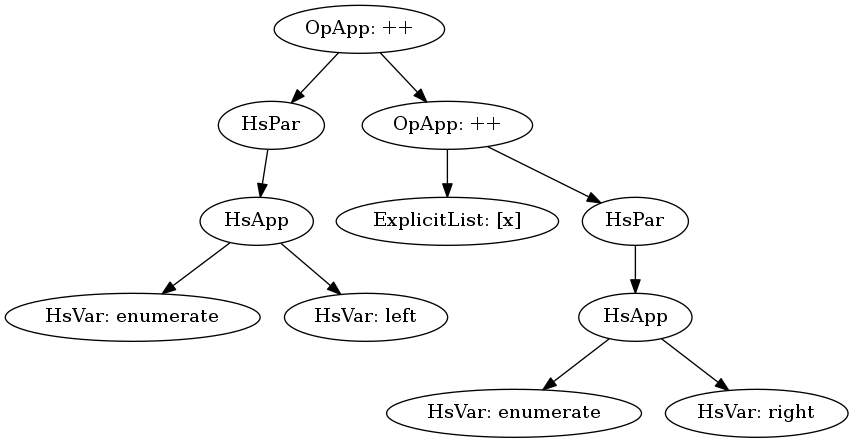
\includegraphics[scale=.5]{graphVis/Chapter3/enumerate.png}
	\end{center}
	\caption{A simplified syntax tree of \texttt{enumerate}'s second case.}
	\label{enumAST}
\end{figure}

The refactoring begins the traversal at the top of the syntax tree with the goal of modifying the entire tree to have a result type of \texttt{DList a}. The root node of the tree is the operator application of the left-hand append operation. This append's result type is the type that determines the whole tree's result type. The standard append operation is paired with the difference list \texttt{DL.append} operation. The refactoring checks to ensure that the difference list append has the correct result type and because it does makes the replacement.\footnote{The refactoring will automatically make \texttt{DL.append} infix by surrounding the call with backtick characters since this replacement is modifying an operator application.} After replacing \texttt{++} with \texttt{DL.append} the result type is correct but the function will no longer type check because \texttt{++} and \texttt{DL.append}'s arguments are not the same types. 

The refactoring then must recurse down both the left and right subtrees to change their types from \texttt{[a]} (the type of \texttt{(++)}'s arguments) to \texttt{DList a} (the type \texttt{append}'s arguments). 

\begin{figure}[h]
	\begin{center}
		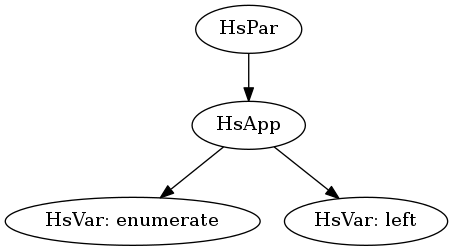
\includegraphics[scale=.5]{graphVis/Chapter3/enumLeft.png}
	\end{center}
	\caption{The left subtree of \texttt{enumerate}'s second case.}
	\label{enumLeft}
\end{figure}

The left subtree of the root node is shown in figure~\ref{enumLeft}. The refactoring can descend through the parentheses (represented by the \texttt{HsPar} constructor); the refactoring continues down the left side of the function application (\texttt{HsApp}). When the refactoring encounters the call to \texttt{enumerate} it recognises that this is the recursive call and even though the type of \texttt{enumerate} stored in the syntax tree is \texttt{Tree a -> [a]} after the refactoring its type will be \texttt{Tree a -> DList a} which is the correct result type  for this subtree. The refactoring can now confirm that the left subtree is of type \texttt{DList a} without checking the right side of the application because the refactoring didn't change the type of \texttt{enumerate}'s arguments.

\begin{figure}[h]
	\begin{center}
		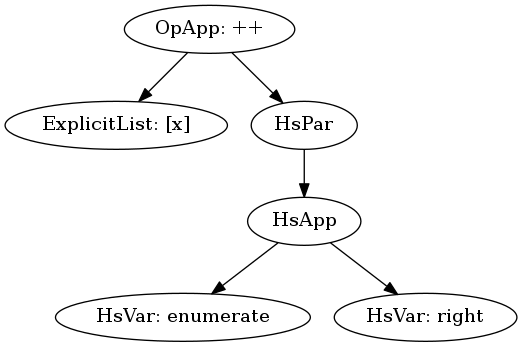
\includegraphics[scale=.5]{graphVis/Chapter3/enumRight.png}
	\end{center}
	\caption{The right subtree of \texttt{enumerate}'s second case.}
	\label{enumRight}
\end{figure}

After refactoring the left subtree the right subtree needs to be modified to be of type \texttt{DList a} as well. Shown in figure~\ref{enumRight}, the right subtree's root is the second call to \texttt{(++)}. Once again the refactoring replaces \texttt{++} with \texttt{DL.append} because \texttt{append}'s result type is also \texttt{DList a}. Doing this replacement sets off additional traversals that need to ensure that the two arguments to the root node become typed \texttt{DList a} as well. The right argument to the root of this subtree is the \texttt{(enumerate right)} expression which is handled in the same way the \texttt{(enumerate left)} call was handled. The left subtree of figure~\ref{enumRight}  is the list literal \texttt{[x]}. This can be replaced with a call to \texttt{(DL.singleton :: a -> DList a)} the equivalent difference list function. At this point the refactoring is finished modifying \texttt{enumerate} and the result can be seen in listing~\ref{enumRef}.

\begin{figure}[t]
\begin{lstlisting}
enumerate :: Tree a -> DList a
enumerate Leaf = empty
enumerate (Node left x right) = (enumerate left) `append` (singleton x) `append` (enumerate right)
\end{lstlisting}
\caption{The refactored definition of \texttt{enumerate}}
\label{enumRef}
\end{figure}

The refactoring isn't finished yet, however. The original definition contained in figure~\ref{enumBefore} had another function \texttt{printEnumTree} that depended on \texttt{enumerate}. The final modification that needs to happen to this example is to wrap all calls to \texttt{enumerate} in \textit{non-refactored} definitions with the abstraction function to convert the result back to a list. The final product of the refactoring can be seen in figure~\ref{enumFinal}.

\begin{figure}[t]
\begin{lstlisting}
data Tree a = Leaf
            | Node (Tree a) a (Tree a)

enumerate :: Tree a -> DList a
enumerate Leaf = empty
enumerate (Node left x right) = (enumerate left) `append` (singleton x) `append` (enumerate right)

printEnumTree :: (Show a) => Tree a -> IO ()
printEnumTree tree = let lst = toList (enumerate tree) in
  print lst
\end{lstlisting}
\caption{The final product of the refactoring}
\label{enumFinal}
\end{figure}

\subsection{Modifying Parameter and Result Types}

The final case of this refactoring involves modifying both the result type and one (or more) of the parameters of the target function. This example will use the \texttt{explode} function from figure~\ref{explode} to refactor both its argument and result type to become \texttt{DList a}.

\begin{figure}[t]
\begin{lstlisting}
explode :: [a] -> [a]
explode lst = concat (map (\x -> replicate (length lst) x) lst)
\end{lstlisting}
\caption{The initial definition of \texttt{explode}}
\label{explode}
\end{figure}

The abstract syntax tree of \texttt{explode} is in figure~\ref{explode}.

\begin{figure}[h!]
	\begin{center}
		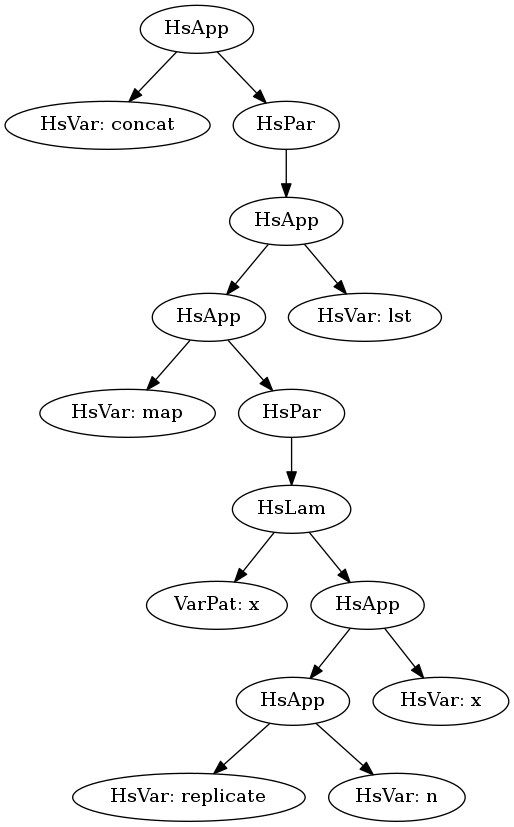
\includegraphics[scale=.5]{graphVis/Chapter3/explode.png}
	\end{center}
	\caption{A simplified representation of \texttt{explodes}'s syntax tree}
	\label{explode}
\end{figure}

Much like the previous case where just the result type was modified, the refactoring will start working on the syntax tree in a top-down manner modifying the function definition to have the correct result type. This case could also be implemented in a bottom-up manner the top-down method allows for more code reuse from the implementation of the case when the result type is modified.

The refactoring starts on the left subtree with the call to \texttt{concat :: Foldable t => t [a] -> [a]}. The equivalent difference list function is \texttt{DL.concat :: Foldable t => t (DList a) -> DList a} since the result type of this version of \texttt{DL.concat} is \texttt{DList a} the refactoring performs the switch between which function to use. 

After the change on the left subtree the refactoring needs to modify the right subtree so that it is of type \texttt{Foldable t => t (DList a)} rather than its current type of \texttt{Foldable t => t [a]}. The leftmost child of the right subtree is the call to \texttt{map :: (a -> b) -> [a] -> [b]}. The difference list equivalent map is appropriately typed \texttt{DL.map :: (a -> b) -> DList a -> DList b}. Should the refactoring change this node to the difference list version? And if so what changes will be need to made to other subtrees?

The refactoring will swap this node out if \texttt{Foldable t => t (DList a)} (the type of \texttt{DL.concat}'s parameter) can be the same type as \texttt{DList b} (\texttt{DL.map}'s result type); since \texttt{DList} is a member of the \texttt{Foldable} type class the swap can happen as long as the \texttt{b} type variable in \texttt{map}'s type is equal to \texttt{DList a}. This node's type after the swap and filling in the known type variables is: \texttt{DL.map :: (a -> DList b) -> DList a -> DList (DList b)} this new type's arguments' types are both different from the original types so the refactoring will need to check both of these subtrees as well. 

\begin{figure}[h]\label{explodeLam}
	\begin{center}
		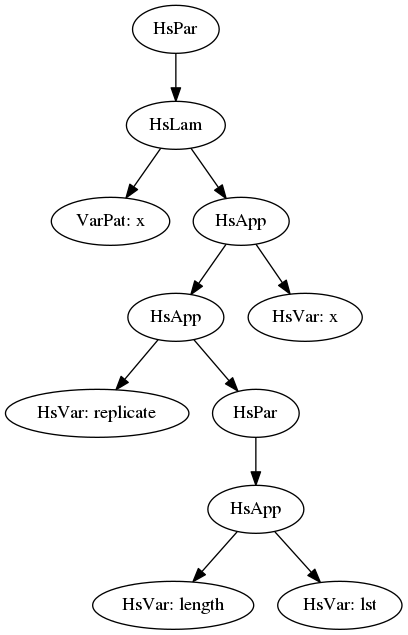
\includegraphics[scale=.5]{graphVis/Chapter3/explodeLam.png}
	\end{center}
	\caption{The syntax tree of the lambda expression in \texttt{explode}.}
\end{figure}

Starting with the lambda expression (the syntax tree in figure~\ref{explodeLam}) the refactoring needs to modify it's type to become \texttt{a -> DList b}\footnote{\texttt{a} and \texttt{b} could be the same type.}. The current type of the lambda expression is \texttt{a -> [a]} so the refactoring only needs to modify its result type. The refactoring can then proceed to the left-most child of this expression, the call to \texttt{replicate :: Int -> a -> [a]}. The refactoring swaps this call for the difference list version of \texttt{DL.replicate :: Int -> a -> DList a}. 

If this refactoring were only modifying the result type of \texttt{explode} the refactoring would be done modifying the lambda expression because the type change affects the syntax tree in a top down manner. In this case, however, because  the type of \texttt{explode}'s argument was also changed so leaves of the syntax tree can also have changed type. This means that every subtree needs to be checked to ensure that it still type checks.

The untouched sections of this expression's syntax tree are \texttt{replicate}'s arguments. The second argument is just the variable \texttt{x} which hasn't changed type. The first argument on the other hand is the expression \texttt{(length lst)} and \texttt{lst} is the argument of \texttt{explode} that is now a difference list rather than a normal list. Ideally the refactoring would rewrite this expression by replacing the normal list functions (\texttt{length} in this case) with difference list equivalents. Unfortunately there is no difference list version of \texttt{length} so the refactoring will have to introduce the abstraction function to convert back to a normal list to calculate its length. 

The lambda expression has now been successfully refactored. The rewritten lambda expression is in figure~\ref{lamRef}.\footnote{To help clarify which functions are for lists and which are the difference list versions, all difference list functions have been qualified with the \texttt{DList} identifier.}

\begin{figure}[t]
\begin{lstlisting}
(\x -> DList.replicate (length (DList.toList lst)) x)
\end{lstlisting}
\caption{The refactored lambda expression.}
\label{lamRef}
\end{figure}


Once refactoring the lambda expression is finished there is only a single node of \texttt{explode} that the refactoring hasn't touched yet, the use of \texttt{lst} as the second argument of \texttt{map}. When the refactoring swapped \texttt{map} for its difference list version it was able to determine the new type of both its arguments, \texttt{(a -> DList b)} for the first argument (the lambda expression) and \texttt{DList a} (\texttt{lst}). Fortunately because \texttt{lst} is a target of the refactoring its new type is \texttt{DList a} so this node can remain unchanged.

\begin{figure}[t]
\begin{lstlisting}
import qualified Data.DList as DL
import Data.DList (DList)

explode :: DList a -> DList a
explode lst = DL.concat 
	(DL.map 
		(\x -> DL.replicate (length (DL.toList lst)) x) 
		lst)
\end{lstlisting} 
\caption{The final refactored result of \texttt{explode}.}
\label{explodeFinal}
\end{figure}

The final result of this case of the Hughes list refactoring is in listing~\ref{explodeFinal}.

\section{Summary}

This chapter has introduced the concept of data-driven refactorings for the object-oriented programming paradigm and described three of the data-driven refactorings developed for this thesis. The first, introducing a type signature, creates additional abstraction to better describe what types are representing. Generalise Maybe takes code written for a specific type and generalises it so that it is applicable to more types. Finally the list to Hughes list refactoring replaces one type with another equivalent type. This refactoring allows a project to be retyped mid-development because it's not always clear from the beginning of a project what the correct data representation should be.

The following chapters will expand on some of these ideas. The next chapter will describe another form of generalisation that rewrites monadic code into its equivalent applicative functor code. The applicative code can be much cleaner and descriptive in certain cases. It can also allow programmers to take advantage of a different way of executing their programs. Chapter~\ref{chap:monadification} discusses introducing effectful abstractions into pure code. This process helps a code base add additional features, such as shared state, mid-development.

\chapter{Implementing Data-Driven refactorings}\label{implementation}

Implementing Data-Driven refactorings have unique challenges. This chapter will discuss the implementation of the refactoring from the previous chapter.

Outline

\begin{itemize}
\item Implementation of Introduce Type Synonym
\item Implementation of Maybe to MonadPlus
\item Implementation of "Isomorphic" refactoring with a focus on the generalisability of the approach.
\end{itemize}

\chapter{Generalising Monads to Applicative}
\label{applicative}

The previous chapter introduced the concept of a functional data refactoring and gave two examples, introducing a type synonym and generalising Maybe to MonadPlus. This chapter will cover another generalising refactoring in more depth, rewriting monadic functions to use applicative functors. 

In their 2008 functional pearl "Applicative programming with effects" Conor McBride and Ross Paterson introduced a new typeclass that they called Idioms but are also known as Applicative Functors~\citep{mcbrideIdioms}. Idioms provide a way to run effectful computations and collect them in some way. They are more expressive than functors but more general than Monads, further work was done in~\citep{arrowsAndIdioms} to prove that Idioms are also less powerful than Arrows.

Applicative functors were implemented in GHC as the typeclass \texttt{Applicative}. An interesting part of the history of GHC is that despite McBride and Paterson proving in their original functional pearl that all monads are also applicative functors, however,  GHC did not actually require instances of monad to also be instances of Applicative until GHC's 7.10.1 release~\citep{ghc7.10Release}. Now that every monad must also be an applicative functor there now exists a large amount of code which could be rewritten using the applicative operators rather than the monadic ones. 

This chapter will discuss the design and implementation of a refactoring which will automatically refactor code written in a monadic style to use the applicative operators instead. Section~\ref{sec:appOverview} is a brief overview of the \texttt{Applicative} typeclass's operators, section~\ref{sec:appProgStyle} will discuss the applicative programming style and, in general, how programs are constructed using the applicative operators, next, section~\ref{sec:appApps} will cover some common applications of this refactoring, section~\ref{sec:appRefact} will specify the refactoring itself, section~\ref{sec:appPrecons} covers the preconditions of the refactoring, finally section~\ref{sec:appVariations} outlines other refactorings that may be used in conjunction with the generalising monads to applicative refactoring and some possible variations of this refactoring. 

\section{The Applicative Typeclass}
\label{sec:appOverview}

The \texttt{Functor} typeclass defines a single function that must be implemented, \texttt{fmap}.

\begin{lstlisting}[frame=tblr]
class Functor f where
	fmap :: (a -> b) -> f a -> f b
\end{lstlisting}

The \texttt{fmap} function allows for a function to be applied to the contents of the Functor f. One could think of the functor as a context and \texttt{fmap} as a function that allows other functions to run within that context. However, what if you wanted to chain together sequences of commands within that context? This is not possible with just functors since \texttt{fmap} does not have the function inside of the functor's context. Sequencing commands will require a more powerful abstraction, applicative functors~\citep{realWorldHaskell}. 

In Haskell applicative functors are implemented in the \texttt{Applicative} typeclass. \texttt{Applicative} typeclass declares two functions, \texttt{pure} and \texttt{(<*>)}. The types of these two functions are shown in listing~\ref{appTypes} where \texttt{f} is the applicative functor. 

\begin{lstlisting}[frame=tblr,label=appTypes,caption={Types of Applicative's minimal complete definition}]
pure :: a -> f a
(<*>) :: f (a -> b) -> f a -> f b
\end{lstlisting}

The \texttt{pure} function is the equivalent of monad's \texttt{return}, it simply lifts a value into the applicative context. The other function \texttt{(<*>)} (which is typically pronounced "applied over" or just "apply"). Apply take in two arguments, both of which are applicative values. The first argument is function within an applicative context from types a to b, and the second argument is of type a. Apply returns a value of type b inside of the same functional context. Apply "extracts" the function from the first argument and the value from the second argument and applies it to the function, all within whatever the applicative context is.

\subsection{Other useful functions}

Though \texttt{pure} and apply are the only two functions that are required to be defined to declare an instance of applicative there are several other useful functions that can either be derived from these two functions or come from other typeclasses which will be briefly covered here. First there are two variations on apply.

\begin{lstlisting}[frame=tblr]
(*>) :: f a -> f b -> f b
(<*) :: f a -> f b -> f a
\end{lstlisting}

These functions sequence actions and still perform the contextual effects of both of their arguments but discard the value of the first and second argument respectively. These functions are used when some operation affects the applicative context but their returned value will not affect the final result of the applicative expression. For example when writing parsers it is common to have to consume some characters from the input without those characters affecting the final result of the parser.

A consequence of the applicative laws is that every applicative's functor instance will satisfy the following~\citep{control.applicative}: 

\begin{lstlisting}[frame=tblr]
f <$> x = pure f <*> x
\end{lstlisting}

The next section will cover how these functions can be used in an applicative style of programming. 

\section{The Applicative Programming Style}
\label{sec:appProgStyle}

In~\citep{mcbrideIdioms} the authors prove that any expression built from the applicative combinators can take the following canonical form:

\begin{lstlisting}[frame=tblr]
pure f <*> is_1 <*> ... <*> is_n
\end{lstlisting}


Where some of the \texttt{is}'s have the form \texttt{pure s} for a pure function \texttt{s}. Due to the rule mentioned at the end of the previous section this canonical form can also be expressed using the infix version of fmap \texttt{(<\$>)}. 

\begin{lstlisting}[frame=tblr]
f <$> is_1 <*> ... <*> is_n
\end{lstlisting}

This is the form that most programs will take when they are refactored from a monadic style. 


 Context-free parsing is a good use case of the applicative type and many examples in this chapter are taken from parsers defined using the parsec library~\citep{parsec}. The first example of the applicative programming style is a function that parses money amounts of the form \texttt{<currency symbol><whole currency amount>.<decimal amount>} e.g. "\$4.59" or "\textsterling64.56".
 
 \begin{lstlisting}[frame=tblr]
 data Currency = Dollar
                          | Pound
                          | Euro
              
data Money = M Currency Integer Integer

parseMoney :: CharParser () Money
parseMoney = M <$> parseCurrency <*> readWhole <*> readDecimal
 \end{lstlisting}
 
The \texttt{parseMoney} function is in the canonical form as defined by~\citep{mcbrideIdioms}. The pure function \texttt{M} is lifted into the \texttt{CharParser} context and its three arguments are provided by three smaller parsers that handle the currency symbol, the whole amount, and the decimal amount separately. 

The only difference between \texttt{readWhole} and \texttt{readDecimal} is that \texttt{readDecimal} has to consume the decimal point before reading the number. Instead of duplicating that number code let's perform a small refactoring to lift the parsing of the decimal into the \texttt{parseMoney} function which will allow us to reuse the \texttt{readWhole} function.

 \begin{lstlisting}[frame=tblr]
parseMoney :: CharParser () Money
parseMoney = M <$> parseCurrency <*> readWhole <* char '.' <*> readWhole
 \end{lstlisting}
 
 Here we can see that the result of parsing the decimal point is discarded because of the use of \texttt{<*} rather than the full apply. All of the variations of apply are left associative so the following definition of \texttt{parseMoney} causes a type error.
 
  \begin{lstlisting}[frame=tblr]
parseMoney :: CharParser () Money
parseMoney = M <$> parseCurrency <*> readWhole <*> char '.' *> readWhole
 \end{lstlisting}
 
This error can be corrected by wrapping "\texttt{char \textquotesingle.\textquotesingle~*> readWhole}" in parenthesis. 
 
The canonical style of applicative functions is not always the most idiomatic way to define things. The following function parses strings surrounded by double quotes.

\begin{lstlisting}[frame=tblr]
parseStr :: CharParser () String 
parseStr = char '"' *> (many1 (noneOf "\"")) <* char '"'
\end{lstlisting}

\texttt{parseStr} does not match the canonical form because no lifted pure function is applied to the rest of the applicative chain. This function could be transformed to canonical form by pre-pending "\texttt{id <\$>}."

The examples covered in this section give a basic introduction to programming in an applicative style. The next section will discuss common applications that are particularly well suited to definition in the applicative style and can be transformed from the monadic style. 

\section{Applications of the Refactoring}
\label{sec:appApps}

There are two things that make a particular application a good candidate for this refactoring. First, and most obviously, the application must be able to be defined using the applicative interface. Finally a good candidate will already have a large corpus of code that is already written in the monadic style. If a particular library already encourages its users to use it using applicative functors rather than monads then there is little work for the refactoring to do.

\subsection{Parsec}
Parser combinator libraries such as parsec~\citep{parsec} provide a simple way of building parsers from predefined smaller parsers (a.k.a. the combinators). The applicative interface is sufficient for defining parsers of context-free languages\footnote{This is mostly true. The applicative interface can parse context-sensitive languages if your grammar is an infinite size~\citep{appContextSens}.}. Despite this much of the code written using Parsec is monadic. A good example of this comes from Real World Haskell~\citep{realWorldHaskell}.

\begin{lstlisting}[frame=tblr]
csvFile :: GenParser Char st [[String]]
csvFile = 
    do result <- many line
       eof
       return result
\end{lstlisting}

This can be very simply rewritten using the applicative like so:

\begin{lstlisting}[frame=tblr]
csvFile :: GenParser Char st [[String]]
csvFile = many line <* eof 
\end{lstlisting}      
 
 Shorter code is not always better however, in this case,  I would argue that the applicative style is easy to clearer. The parser can be read left to right many lines are followed by the end of file.
 
\subsection{Yesod}
Another possible application of this refactoring applies to parts of code used to define Yesod webservers~\citep{yesod}. The preferred way to handle the creation and processing of web forms is using the applicative interface~\citep{yesodBook}. Yesod doesn't force forms to be handled applicatively because a monad instance is provided as well but it is the \textit{idiomatic} way to handle web forms. This refactoring would allow people to write in a monadic style and then refactor their code to fit the standard.

\subsection{Other applications}
\comment{Complete section conclusion here}
  

\section{Refactoring Monadic Programs to Applicative}
\label{sec:appRefact}
This section will cover the mechanics of refactoring monadic code to the applicative style. Many of these examples are taken from the parser for money amounts and a JSON parser. The full source of these parse can be found in~\citep{moneyParse} and~\citep{jsonParser}.

Take for example the following parser that parses strings that begin and end with double quotes.

\begin{lstlisting}[frame=tlrb]
parseStr :: CharParser() String
parseStr = do
	char '"'
	str <- many1 (noneOf "\"")
	char '"'
	return str
\end{lstlisting}

This parser first consumes a double quote (\texttt{char \textquotesingle"\textquotesingle}) then parses at least one other character other than double quotes and assigns those characters to the variable named \texttt{str}\footnote{This line is composed of two parser combinators, \texttt{many1}, and \texttt{noneOf}. \texttt{many1} takes another parser as its argument and applies it one or more times returning a list of the results. \texttt{noneOf} takes in a list of characters and succeeds if the current character is not in the provided list. Then the character is returned.}, finally the closing quote is consumed and \texttt{str} is returned. This particular function can be rewritten in an applicative style like so:

\begin{lstlisting}[frame=tlrb]
parseStr :: CharParser() String
parseStr = char '"' *> (many1 (noneOf "\"")) <* char '"'
\end{lstlisting}

The refactoring goes through the monadic version of the function line by line and composes computations with the applicative operators. In this case the first line of the \texttt{do} block does not affect the final result so it is followed by the \texttt{*>} which performs the action on the left hand side of the operator but discards that value. The next line's value is assigned to the variable str which is returned by the function so this means that on both sides of this computation the operator that composes it with its neighbours will have to "point" to it as well\footnote{This means \texttt{<*>} could occur on both sides, \texttt{*>} on the left, or \texttt{<*} on the right of the computation}. To determine which operator needs to be used on the right of the call to \texttt{many1} the refactoring needs to look at the next line and see if it also contributes a value to the final result. If it does then it and \texttt{many1} will be composed by the \texttt{<*>} operator, but since \texttt{char} doesn't, the operator between the call to \texttt{many1} and the second call to \texttt{char} becomes \texttt{<*} which discards the value \texttt{char} returns.

This is a fairly simple function to convert to applicative style. Let's look at another example that adds in more complexity by having multiple computations that contribute to the final value of the function. This function comes from the money parser that was used in~\ref{sec:appProgStyle} as well. 
\pagebreak
\begin{lstlisting}[frame=tlrb]
parseMoney :: CharParser () Money
parseMoney = do
   currency <- parseCurrency 
   whole <- many1 digit
   decimal <- (option "0" (do { 
                           char '.';
                           d <- many1 digit;
                           return d}))
   return $ M currency (read whole) (read decimal)
\end{lstlisting}

The \texttt{parseMoney} function parses text into the \texttt{Money} data type. It works by first consuming the currency symbol and getting the appropriate \texttt{Currency} type from that. Then the whole money amount is read from one or more digits. Finally an "option" parser attempts to match a decimal point followed by one or more digits. If that fails then the decimal amount is zero. These three values are then combined into type \texttt{Money} which is returned. \texttt{parseMoney} can be rewritten in an applicative style like so\footnote{The where clause in this example has been included for formatting and readability and would not be generated automatically.}:

\begin{lstlisting}[frame=tlrb]
parseMoney :: CharParser () Money
parseMoney = M <$> parseCurrency <*> readWhole <*> readDecimal
          where readWhole = read <$> many1 digit
                  readDecimal = read <$> option "0" (do { 
                           char '.';
                           d <- many1 digit;
                           return d}))
\end{lstlisting}

On the left hand side of the chain of applicative actions there is a call to a pure operation, in this case the constructor \texttt{M}. Any pure computations that "collect" the values returned from applicative computations will appear on the left of the chain of operations. The pure computations are composed with applicative computations with the \texttt{<\$>} operator which lifts the computation into the applicative context. The three computations are composed together with the \texttt{<*>} operator because they all contribute to the final result of \texttt{parseMoney}.

The chains of applicative computations can get more complicated. The following snippet of code parses a single in a JSON object which consists of a string key and a value which can be any valid JSON value, separated by a colon, and stores the key and value in a tuple. 

\begin{lstlisting}[frame=tblr]
objEntry = (,) <$> (spaces *> parseStr <* spaces <* char ':' <* spaces) <*> (parseJVal <* spaces)
\end{lstlisting}

When there are a large amount of computations that do not affect the final value of the function as a whole there can be multiple valid ways the chain can be structured. The \texttt{objEntry} function can be defined in several different ways as shown below.

\begin{lstlisting}[frame=tblr]
objEntry = (,) <$> (spaces *> parseStr <* spaces <* char ':') <*> (spaces *> parseJVal <* spaces)

objEntry = (,) <$> (spaces *> parseStr) <*> (spaces *> char ':' *> spaces *> parseJVal <* spaces)
\end{lstlisting}

Both of the above versions of \texttt{objEntry} are equivalent to the first version. The automated refactoring will produce the first version of \texttt{objEntry}. The refactoring in general will produce applicative chains according to the following rules. Both sides of the apply operator will be parenthesised statements. After the first value producing operation every side effect causing operation will be composed with \texttt{(<*)}. In general the produced applicative chain will take the following form.

\begin{lstlisting}[frame=tblr]
f = pf <$> (is_1 *> ... is_n *> vs_1 <* js_1 ... <* js_n) <*> (vs_2 <* ks_1 ... <* ks_n) ... <*> (vs_n ...)
\end{lstlisting}

The \texttt{vs} are functions that return values to be passed to the pure function \texttt{pf} all other functions just run within the applicative context without affecting the returned value of \texttt{f}.

\section{Preconditions of the Refactoring (When is a Monad actually a Monad?)}
\label{sec:appPrecons}

Many functional refactorings have non-trivial preconditions that must hold before the refactoring can be applied~\citep{refacTools}. Fortunately this refactoring only has a single fairly simple precondition, the function to be refactored must be definable with the applicative interface not just the monadic interface. What does this mean exactly? Where is the line between applicative and monadic? Let's start by looking at the type signatures of the bind and apply functions.

\begin{lstlisting}[frame=tblr]
(<*>) :: Applicative f => f (a -> b) -> f a -> f b

(>>=) :: Monad m => m a -> (a -> m b) -> m b
\end{lstlisting}  

One thing to keep in mind is that these two functions' arguments are in opposite order. The key difference becomes clearer when examining the type of apply when its arguments are flipped.

\begin{lstlisting}[frame=tblr]
flip (<*>) :: Applicative f => f a -> f (a -> b) -> f b
\end{lstlisting}

The only difference between this version of apply and bind is in the second argument. Bind takes in a function that takes in a value of type \texttt{a} and returns an \texttt{m b} whereas apply receives an applicative functor that contains a function from \texttt{a} to \texttt{b}. This means that within a monadic context bind allows access to the pure value contained in the monad while all of the arguments to apply are contained within the applicative functor.

What does this mean in practice? For example, the following functions are taken from a StackOverflow answer by Conor McBride~\citep{soApp}.

\begin{lstlisting}[frame=tblr]
iffy :: Applicative a => a Bool -> a x -> a x -> a x
iffy ab at af = pure cond <*> ab <*> at <*> af where
  cond b t f = if b then t else f

miffy :: Monad m => m Bool -> m x -> m x -> m x
miffy mb mt mf = do
  b <- mb
  if b then mt else mf
\end{lstlisting} 

Both of these functions attempt to implement an if statement, \texttt{iffy} does it with \texttt{pure} and \texttt{(<*>)} whereas \texttt{miffy} uses the monadic functions. Both functions' first argument contains a boolean within its computational context. Depending on the value of this boolean the second or third argument is then returned. Though both of these functions will return the same value when given the same arguments, the effects within the context will be very different. When \texttt{iffy} is run all of the contextual effects will be run regardless of which value is returned.

If a value retrieved from the monadic context is used in a right hand side expression before the return statement then that function cannot be refactored to use the applicative interface without changing the contextual effects of the function. 

\section{Variations and Related Refactorings}
\label{sec:appVariations}

This section will discuss related refactorings and variations on the generalise monad to applicative refactoring that may be useful. Related refactorings help transform code so that it can pass the preconditions. In this case it may be possible to extract monadic code into another function making the top level function definable with the applicative interface. Variations on refactorings slightly change the behavior of the refactoring. This section will present two variations, one which will inline small do blocks of monadic code automatically, another will
recursively refactor do blocks that may occur inside of higher level statements.

\subsection{Extract monadic code}
\label{subSec:extract}
Say someone wanted to refactor the following code to use the applicative interface rather than the monadic one it currently uses.

\begin{lstlisting}[frame=tblr]
f = do
	x <- getX
	b <- getB
	y <- if b then getY1 else getY2
	log y
	return (x,y)	
\end{lstlisting}

This code will not pass the precondition because both \texttt{b} and \texttt{y} are used on the right as well as the left hand side of the equation. However, lines three through five don't really affect the rest of the function so they could be refactored into their own function then f could be rewritten applicatively.

\begin{lstlisting}[frame=tblr]
f = (,) <$> getX <*> g

g = do
	b <- getB
	y <- if b then getY1 else getY2
	log y
	return y
\end{lstlisting}

\subsection{Inline do blocks}
Instead of extracting an entire function as in subsection~\ref{subSec:extract} a developer may prefer to just inline a do block. This is useful if the monadic section is fairly small.

\begin{lstlisting}[frame=tblr]
f = do
	x <- result1
	y <- result2
	z <- result3
	log z
	return (x,y)
\end{lstlisting}
\larger[5]
\[\Rightarrow\]
\normalsize
\begin{lstlisting}[frame=tblr]
f = (,) <*> result1 <*> (result2 <* do{z <- result3; log z})
\end{lstlisting}

Normally the variable \texttt{z} would prevent the function from being refactored. Introducing the small do block allows for a simple readable applicative function to be produced. 

It is worth noting that if the variable \texttt{z} was also included in the output of the function the do block inlining would still work with a slight modification.

\begin{lstlisting}[frame=tblr]
f = (,) <*> result1 <*> result2 <*> do{z <- result3; log z; return z}
\end{lstlisting}

\subsection{Refactor Inner \texttt{do} blocks}
If we take another look at the \texttt{parseMoney} function and it's applicative counterpart the default behaviour of the refactoring preserves the inner do block passed to the \texttt{option} parser.

\begin{lstlisting}[frame=tlrb]
parseMoney :: CharParser () Money
parseMoney = do
   currency <- parseCurrency 
   whole <- many1 digit
   decimal <- (option "0" (do { 
                           char '.';
                           d <- many1 digit;
                           return d}))
   return $ M currency (read whole) (read decimal)
   
parseMoney :: CharParser () Money
parseMoney = M <$> parseCurrency <*> readWhole <*> readDecimal
          where readWhole = read <$> many1 digit
                  readDecimal = read <$> option "0" (do { 
                           						char '.';
                          						d <- many1 digit;
                           						return d}))
\end{lstlisting}

It is perfectly possible to refactor this inner do block to the applicative style as well.

\begin{lstlisting}[frame=tblr]

parseMoney :: CharParser () Money
parseMoney = M <$> parseCurrency <*> readWhole <*> readDecimal
          where readWhole = read <$> many1 digit
                  readDecimal = read <$> option "0" (char '.' *> many1 digit)
\end{lstlisting}


\chapter{Introducing Monads}\label{chap:monadification}
Up to this point the data refactorings that have been discussed are changing abstractions that already existed in the source code. This chapter will explore refactorings that introduce effectful abstractions into pure code. In particular this chapter will focus monadification, the process of adding monads to pure code. 

Monadification of a Haskell program is a common transformation that must be performed if a problem becomes more complicated than is easily expressed without them\footnote{I've had a colleague remark to me: "I can't 
count the number of times I've been in the middle of something and realized I needed some state."}. The Haskell communities guidelines also advise that monadic and pure code should be separated if possible so Haskell programs should be written as pure code until it is certain that monads are required~\citep{guidelines}. This makes the process of monadification a common transformation that Haskell programs undergo, making it a compelling refactoring target.

This chapter will describe a monadification refactoring. First will be a very brief definition of the \texttt{Monad} type class from GHC. There are multiple styles of monadification as described in~\citep{monadSurvey} and this chapter will describe these styles and discuss their relative merits and usefulness to the Haskell community. Finally the chapter will describe the implementation of monadification within the HaRe project.
 
\section{The Monad Typeclass}

The monad typeclass as it exists in GHC is defined in figure~\ref{monadDef}. The two canonical monad functions are \texttt{return} and bind (\texttt{(>>=)}). \texttt{return} is the function that brings some pure value into the monadic context the default definition is the function \texttt{pure} from the applicative instance of the type. Bind allows for computation to occur within the monadic context.

\begin{figure}[t]
\begin{lstlisting}
class Applicative m => Monad m where
	(>>=) :: m a -> (a -> m b) -> m b

	(>>) :: m a -> m b -> m b
	m >> k = m >>= \_ -> k
	
	return :: a -> m a
	return = pure
	
	fail :: String -> m a
	fail s = errorWithoutStackTrace s
\end{lstlisting}
\caption{The monad typeclass}
\label{monadDef}
\end{figure}

The other two functions are provided by the GHC implementation of the type class. The \texttt{(>>)} operator allows for composing together functions where the second operation is not dependent on the outcome of the first. \texttt{fail} is called when a pattern match failure occurs inside of a \texttt{do} statement. In figure~\ref{failCall} \texttt{fail} would be called if the function \texttt{f} returns a \texttt{Nothing} rather than a \texttt{Just}.

\begin{figure}[t]
\begin{lstlisting}
do{
(Just n) <- f;
return (n+1)
}
\end{lstlisting}
\caption{A \texttt{do} statement with a possible call to \texttt{fail} on line 2.}
\label{failCall}
\end{figure}

\section{Styles of Monadification}

Up to this point this thesis has been fairly vague about what monadification is beyond the process of introducing monads into a previously pure type. Monadifying a single type changes it from type \texttt{a} to type \texttt{Monad m => m a}. Monadifying a function on the other hand changes the result type of the function because there is no way to extract values out of any given monadic context. Monadification can also affect any combination of parameters. Which parameters are affected depends on the \textit{style} of monadification.

The different styles of monadification can change how a function is evaluated. In~\citep{monadSurvey} five different styles of monadification are described as part of a survey on the Haskell community's use of monads. The monadification styles are:

\begin{itemize}
\item Full Call-by-Value
\item Full Call-by-Name
\item Restricted Call-by-Name
\item Data-Directed
\item Restricted Call-by Value
\end{itemize}


\subsection{Full Call-by-Value Monadification}

A call-by-value monadification will ensure that all arguments are evaluated before being passed to a function and a function will also be evaluated before having arguments passed to it. Consider the definition of mergesort in figure~\ref{mergesrt}.

\begin{figure}[t]
\begin{lstlisting}
mergesort :: (Ord a) => [a] -> [a]
mergesort lst = let (l,r) = splitAt ((length lst) `div` 2) lst in
	merge (mergesort l) (mergesort r)
	
merge :: (Ord a) => [a] -> [a] -> [a]
merge [] r = r
merge l [] = l
merge (x:xs) (y:ys) = 
	case (x < y) of
	True  -> x:(merge xs (y:ys))
	False -> y:(merge (x:xs) ys)						
\end{lstlisting}
\caption{Mergesort}
\label{mergesrt}
\end{figure}

The full call-by-value monadification when applied to \texttt{mergesort} is defined in figure~\ref{fcbv}

\begin{figure}[t]
\begin{lstlisting}

mergesort :: (Ord a, Monad m) => m ([a] -> m [a])
mergesort = return (\ lst -> case lst of
                 [] -> return []
                 [x] -> return [x]
                 _ -> do
                   let (l,r) = splitAt ((length lst) `div` 2) lst
                   mm1 <- mergesort
                   v1 <- mm1 l
                   mm2 <- mergesort
                   v2 <- mm2 r
                   return (merge v1 v2))					
\end{lstlisting}
\caption{Full call-by-value monadification of mergesort}
\label{fcbv}
\end{figure}

\subsection{Full Call-by-Name Monadification}

The full call-by-name monadification ensures arguments are unevaluated when they are passed to the function. The full call-by-name version of \texttt{mergesort} is defined in figure~\ref{fcbn}.


\begin{figure}[t]
\begin{lstlisting}
mergesort :: (Ord a, Monad m) => m (m [a] -> m [a])
mergesort = return (\ mlst -> do
		lst <- mlst			
		res <- case lst of
                   [] -> return []
                   [x] -> return [x]
                   _ -> do
                     let (l,r) = splitAt ((length lst) `div` 2) lst
                     mm1 <- mergesort
                     v1 <- mm1 (return l)
                     mm2 <- mergesort
                     v2 <- mm2 (return r)
                     return (merge v1 v2)
		return res)					
\end{lstlisting}
\caption{Full call-by-name monadification of mergesort}
\label{fcbn}
\end{figure}

The two "full" monadification styles monadify both the arguments to a function as well as the function itself. The remaining styles are restrictions of these full modifications where only some of the arguments are modified not the functions. 

\subsection{Restricted Call-by-Name Monadification}
This style of monadification is where every argument is contained within the monad. Using the mergesort example again, figure~\ref{resCBN} shows the restricted call-by-name monadification.

\begin{figure}[t]
\begin{lstlisting}
mergesort :: (Ord a, Monad m) => m [a] -> m [a]
mergesort ml = do
	lst <- ml
	res <- case lst of
		[] -> return []
		[x] -> return [x]
		_ -> do 
			let (l,r) = splitAt ((length lst) `div` 2) lst
			v1 <- mergesort (return l)
			v2 <- mergesort (return r)
			return (merge v1 v2)
	return res	
\end{lstlisting}
\label{resCBN}
\end{figure}

All of the arguments to \texttt{mergesort} in figure~\ref{resCBN} are within the monad so the arguments will be evaluated hence the call-by-name "flavour" as~\citep{monadSurvey} describes it.

\subsection{Data-Directed Monadification}
This style refactors a certain type to be replaced by a monadic computation over that type. The example given in~\citep{monadSurvey} is a simple arithmetic expression interpreter as seen in figure~\ref{fig:interpreter}.

\begin{figure}[t]
\begin{lstlisting}
data Expr = Lit Int
	| Bin Op Op Expr Expr

data Op = Add | Div

eval :: Expr -> Int
eval (Lit n) = n
eval (BinOp op e1 e2)
	= evalOp op (eval e1) (eval e2)
	
evalOp :: Op -> Int -> Int -> Int
evalOp Add v1 v2 = v1 + v2
evalOp Div v1 v2 = v1 `div` v2
\end{lstlisting}
\caption{The pure interpreter implementation}
\label{fig:interpreter}
\end{figure}

With this particular example the programmer wants the expressions to be evaluated within a monad to add effects. Since \texttt{Int} represents the result of an expression in this program this type is monadified as seen in figure~\ref{fig:monInterp}. Importantly this refactoring makes the type of \texttt{evalOp} change to \texttt{Monad m => Op -> m Int -> m Int -> m Int} in addition to monadifying the result type of \texttt{eval}. 

\begin{figure}[t]
\begin{lstlisting}
eval :: Monad m => Expr -> m Int
eval (Lit n) = return n
eval (BinOp op e1 e2)
	= evalOp op (eval e1) (eval e2)
	
evalOp :: Monad m => Op -> m Int -> m Int -> m Int
evalOp Add v1 v2 = do 
	l <- v1
	r <- v2	
	return (l + r)
evalOp Div v1 v2 = do
	l <- v1
	r <- v2
	return (l `div` r)
\end{lstlisting}
\caption{A data-directed monadification of the interpreter.}
\label{fig:monInterp}
\end{figure}

Data-directed monadification is useful if a particular type can always represent the result of a computation that should be effectful. In the interpreter case, \texttt{Int} is always the result of an evaluation. Even in the only call to \texttt{evalOp} the second and third arguments are computed from recursive calls to \texttt{eval} so those \texttt{Int} types also represent expression evaluation.

This style of monadification would pair well with the introduce a type synonym refactoring to differentiate types that should be monadified. In the interpreter example if it was anticipated that another \texttt{Int} type that didn't represent the result of an evaluation needed to be added to the program.

\subsection{Restricted Call-by-Value Monadification}

The final monadification style simply monadifies the result type of the target function(s). This is the style of monadification that is produced by the algorithm described in~\citep{monadification} and that is implemented in HaRe as part of this thesis work.

Returning to the mergesort example from earlier in the section the restricted call-by-value monadification implementation of this can be seen in figure~\ref{rCBV}.

This style of monadification meshes nicely with the bind operator which expects functions whose arguments are pure values and returns a monadic type. This style of monadification has been implemented in HaRe and the next section will go into greater detail about the implementation of this refactoring.

\begin{figure}[t]
\begin{lstlisting}
mergesort :: (Ord a, Monad m) => [a] -> m [a]
mergesort lst = do
	let (l,r) = splitAt ((length lst) `div` 2) lst
	v1 <- mergesort l
	v2 <- mergesort r
	merge v1 v2
	
merge :: (Ord a, Monad m) => [a] -> [a] -> m [a]
merge [] r = return r
merge l [] = return l
merge (x:xs) (y:ys) = 
	case (x < y) of
	True -> do 
		rst <- (merge xs (y:ys)) 
		return (x:rst)
	False -> do
		rst <- (merge (x:xs) ys)	
	 	return (y:rst)
\end{lstlisting}
\caption{Restricted call-by-value monadification}
\label{rCBV}
\end{figure}

\section{Implementation of the Monadification Refactoring}

The implementation of Monadification in HaRe is a fairly strait forward top down transformation. The monadification refactoring takes in a list of positions as input. Those positions define where the functions that should be monadified are defined. 

The monadification refactoring works over sets of functions at once. Figure~\ref{fgMon} defines two functions \texttt{f} and \texttt{g} and the two possible monadifications (\texttt{*\_m1} and \texttt{*\_m2}). The \texttt{f\_m1} function is how \texttt{f} would be rewritten if it was the sole target of the refactoring, since the right hand side of \texttt{f} is composed from pure values and non-monadic functions \texttt{f\_m1} is defined by applying \texttt{return} to the original definition of \texttt{f}.

When the refactoring targets both \texttt{f} and \texttt{g} these functions will be rewritten to their "\texttt{*\_m2}" equivalents. In this case \texttt{g} is handled in the same way \texttt{f\_m1} was defined, because it is defined entirely with non-monadic values the new right hand side is just the old one composed with \texttt{return}. The definition of \texttt{f\_m2} is slightly more interesting, however, due to the call to the monadified function \texttt{g\_m2}. The refactored version of \texttt{g} in this scenario produces a monadic value of type \texttt{Monad m => m Int} so a call to this function can no longer be passed to \texttt{(+)}. Instead that whole sub-expression is replaced with a new variable "\texttt{v1}." The result of the, now monadic, computation (\texttt{g\_m2 x}) is bound to this new variable via the bind (\texttt{>>=}) operator and lambda expression. 

 

\begin{figure}[t]
\begin{lstlisting}
f :: Int -> Int
f x = (g x) + 1

g :: Int -> Int
g y = y * 2

f_m1 :: (Monad m) => Int -> m Int
f_m1 x = return ((g x) + 1)

f_m2 :: (Monad m) => Int -> m Int
f_m2 x = g_m2 x >>= (\v1 -> return (v1 + 1))

g_m2 :: (Monad m) => Int -> m Int
g_m2 y = return (y * 2)
\end{lstlisting}
\caption{Possible monadification refactorings for the \texttt{f} and \texttt{g} functions.}
\label{fgMon}
\end{figure} 

\subsection{Preconditions}

There are two preconditions that must be met before this refactoring can be applied. First the target functions must be fully applied at all call points. This allows the refactoring to assume that that the type of a subtree who's leftmost child is a monadified functions is a monadic value and not something of type \texttt{Monad m => a -> m a}. 

\begin{figure}[t]
\begin{lstlisting}
f :: Int -> String -> String
f n str = (take n str, drop n str)


stringHandler :: Maybe Int -> String -> (String, String)
stringHandler mi s = 
	let g = case mi of
		Nothing -> f ((length s) `div` 2)
		(Just i) -> f i
	in g s
\end{lstlisting}
\caption{The \texttt{stringHandler} function will be rejected by the monadification refactoring.}
\label{strHan}
\end{figure}

Like the many of the preconditions for the generalise monads to applicative refactoring other refactorings can help transform programs to pass the preconditions. The \texttt{stringHandler} in figure~\ref{strHan} has calls to \texttt{f} that are not fully saturated. Fortunately $\eta$-expansion can be used to fully saturate the calls to \texttt{f} (see figure~\ref{etaHan}) allowing \texttt{stringHandler} and \texttt{f} to be monadified.\footnote{The original definition of \texttt{stringHandler} could be monadified alone.}

\begin{figure}[t]
\begin{lstlisting}
stringHandler :: Maybe Int -> String -> (String, String)
stringHandler mi s = 
	let g = case mi of
		Nothing -> (\x -> f ((length s) `div` 2) x)
		(Just i) -> (\x -> f i x)
	in g s
\end{lstlisting}
\caption{The new version of \texttt{stringHandler} can be monadified.}
\label{etaHan}
\end{figure}

The second precondition that needs to hold before monadification can take place is that none of the target functions can be called by non-monadic functions. This is due to the fact that a target functions result type will change from some pure value \texttt{a} to a monadic computation over \texttt{a} there is no function that retrieves values out of any given monad so the target function, once it is refactored, will be unusable by non-monadic functions. 

This precondition can't really be avoided for the refactoring to happen the set of target functions will have to be changed. Either all functions that reference a target function become target functions as well or the dependent function is dropped from the refactoring.

\subsection{The Transformation}

Very generally monadifying a function works in four steps.

\begin{enumerate}
\item Replace a monadic sub-expression with a new variable
\item Wrap the modified expression with a lambda that takes in the new variable as an argument
\item Bind the original monadic sub-expression to the lambda
\item Repeat until all monadic expressions are removed from the original definition
\end{enumerate}

The refactoring works over the right hand side of a target function and extracts all monadic sub-expressions first. This is done recursively because monadic calls can be at multiple levels of the syntax tree. Take the function \texttt{f} defined in figure~\ref{simpleMon}. It is the target of monadification along with the functions \texttt{g} and \texttt{h}. 

\begin{figure}[t]
\begin{lstlisting}
f x y = f (h x) (g y)
\end{lstlisting}
\caption{A simple target function for monadification}
\label{simpleMon}
\end{figure}  

\begin{figure}[t]
	\begin{center}
		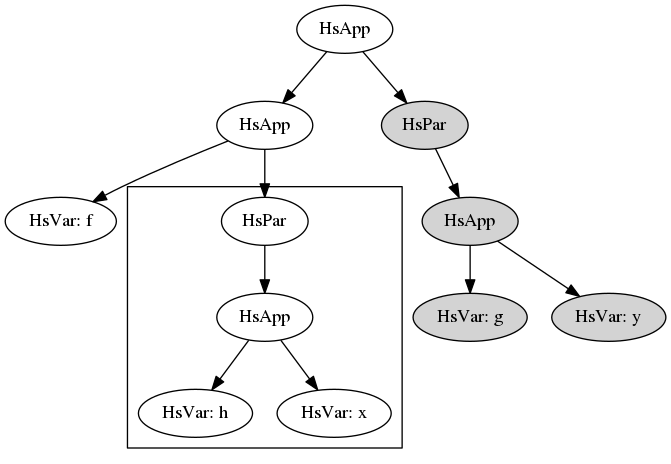
\includegraphics[scale=.5]{graphVis/Chapter6/simpF.png}
	\end{center}
	\caption{The syntax tree of \texttt{f} from figure~\ref{simpleMon}}
	\label{simpF}
\end{figure}

The syntax tree of the right hand side of \texttt{f} is shown in figure~\ref{simpF}. The transformation starts by top down checking the right subtrees for monadic computations. It will first check the call to \texttt{g} (shaded with grey in figure~\ref{simpF}) then it will check the call to \texttt{h} (the corresponding nodes are inside the box). Both of these subtrees are monadic calls so they will be replaced in the tree with unique generated variables. The refactoring implementation contains a queue where the monadic expressions are paired with the variables that replace them and then stored. After this step the expression is \texttt{f v2 v1} and the queue contains two elements \texttt{[(v1,"(g y)"),(v2,"(h x)")]}. The final step checks if the left most child of the current expression is a call to a monadic function. In this case it is because \texttt{f} is a target of the refactoring but if it wasn't then the expression would be composed with \texttt{return}.

At this point the expression is ready to be part of the right hand side of a lambda expression. First element is popped from the queue (in this case it's \texttt{(v1,"g y")}) the variable name that's stored in the element is the argument name in the lambda expression the expression from the queue is composed with the bind operator. In this manner the refactoring keeps popping elements off of the queue wrapping the previous expression in a lambda with the variable name as its argument and composing this lambda with the expression from the queue using bind until the queue is empty.

The final result of refactoring \texttt{f} is shown in figure~\ref{simpF_ref}.

\begin{figure}[t]
\begin{lstlisting}
f x y = (g x) >>= (\ v2 -> (g y) >>= (\v1 -> f v2 v1))
\end{lstlisting}
\caption{The final refactored version of \texttt{f}}
\label{simpF_ref}
\end{figure}

\section{Let Expressions}

The previous section details how the refactoring works over simple function applications. This section will describe how a function with a let expression is refactored. This section will use the expression evaluator in figure~\ref{evalExpr} as a motivating example.

\begin{figure}[t]
\begin{lstlisting}
data Expr = Var Char
          | N Int
          | Add Expr Expr
          | Sub Expr Expr
          | Assign Char Expr
          deriving Show

type Env = [(Char,Int)]

eval :: Expr -> Env -> (Int,Env)

eval (Var v) env = (head [val | (x,val) <- env, x==v], env)

eval (N n) env = (n,env)

eval (Add e1 e2) env = let (v1,env1) = eval e1 env
                                    (v2,env2) = eval e2 env1 
                           in (v1+v2,env2)
eval (Sub e1 e2) env = let (v1,env1) = eval e1 env
                                    (v2,env2) = eval e2 env1 
                           in (v1-v2,env2)
eval (Assign x e) env = let (v,env1) = eval e env 
	in (v, (x,v):env1)
\end{lstlisting}
\caption{An expression evaluator.}
\label{evalExpr}
\end{figure}

The idea is that at this point in the project the explicit passing of the state is unwanted so refactoring \texttt{eval} to become monadic so that the \texttt{Env} can be passed around using the \texttt{State} monad instead. The first two cases that handle the \texttt{Var} and \texttt{N} constructors can simply be wrapped with \texttt{return} because no recursive calls to \texttt{eval} happen in those cases. The three other cases contain let bindings that all call (the now monadic) \texttt{eval}. 

In those cases the local bindings can be used as the variables inside of a lambda expression. This seems simple enough but what order should the bindings be processed in? Consider the let binding in figure~\ref{intLet}, assuming that the \texttt{f} and \texttt{x} variables are in scope, due to lazy evaluation this is a valid Haskell let binding despite \texttt{v1} being referenced on line one before it's defined on line two. However if the let bindings are processed in the obvious way from top to bottom\footnote{In this case: \texttt{g v1 >>= ($\backslash$v2 -> f x >>= ($\backslash$v1 -> ...))}} \texttt{v1} wont be in scope when it's passed to \texttt{g}.  

\begin{figure}[t]
\begin{lstlisting}
let v2 = g v1
     v1 = f x
    in ...
\end{lstlisting}
\caption{An interesting let binding}
\label{intLet}
\end{figure}

Fortunately GHC offers a solution, the renamer does dependency analysis on local bindings and orders them so that later bindings may depend on earlier ones but not vise versa~\citep{ghcApi}. This renamed ordering is used to lookup the parsed bindings in dependency analysed order.

Returning to the evaluator example the monadified version is shown in figure~\ref{monEval}.\footnote{Line breaks have been added to aid readability in this setting but the refactoring would not actually do this.} The let bindings in \texttt{eval} can be processed from top to bottom. In the \texttt{Add} case this means that the expression bound on line 16 in figure~\ref{evalExpr} makes up the outermost call to bind and the pattern it was originally bound to becomes the pattern that matches the argument passed to the first lambda expression. 
\begin{figure}[t]
\begin{lstlisting}
eval :: Monad m => Expr -> Env -> m (Int,Env)

eval (Var v) env = return (head [val | (x,val) <- env, x==v], env)

eval (N n) env = return (n,env)

eval (Add e1 e2) env = eval e1 env >>= 
	(\(v1,env1) -> eval e2 env1 >>= 
		(\(v2,env2) -> return (v1+v2,env2)))

eval (Sub e1 e2) env = eval e1 env >>= 
	(\(v1,env1) -> eval e2 env1 >>= 
		(\(v2,env2) -> return (v1-v2,env2)))

eval (Assign x e) env = eval e env >>= 
	(\(v,env1) -> return (v, (x,v):env1)))
\end{lstlisting}
\caption{The monadified expression evaluator.}
\label{monEval}
\end{figure}

If there were pure expressions on the right hand side of the let binding those bindings will remain in a let expression. For example the function starting on line one in figure~\ref{mixLet} contains two let bindings \texttt{pureF} is a pure function and so it remains inside of a let expression whereas \texttt{monF} is a target of the refactoring and it is lifted from the let and passed to bind. 

\begin{figure}[t]
\begin{lstlisting}
f x = let y = pureF x
             z = monF y
		     in z+x

f_m x = let y = pureF x in
		monF y >>= (\z -> return z+x)
\end{lstlisting}
\caption{A function with a mixture of pure and monadic function calls in a let expression.}
\label{mixLet}
\end{figure}

\section{Sugaring}

The refactored program from figure~\ref{monEval} is rewritten in a restricted call-by-value monadification style. However, idiomatic monadic Haskell is not often written in this style. Haskell also supports a piece of syntactic sugar called \texttt{do} notation. This notation allows for a series of bind computations to be written in a more compact and easier to read style. Figure~\ref{doEx} shows how the bind expression on line one can be sugared into the do statement on lines four through six.

\begin{figure}[t]
\begin{lstlisting}
m_expr >>= (\x -> return (f x))
--Sugars to

do
	x <- m_expr
	return (f x)
\end{lstlisting}
\caption{An example of how binds can sugar to \texttt{do} notation.}
\label{doEx}
\end{figure}

\textbf{\texttt{do}} notation is highly used when writing monadic Haskell programs and some texts even introduce it before explaining what monads are (see \cite{realWorldHaskell} and \cite{learnYou}). Supporting this syntax is an important feature for a monadification refactoring to be practical. 

The sugaring of bind syntax into \texttt{do} syntax is a separate refactoring in HaRe. This allows for the programmer to choose exactly which functions should be written with \texttt{do} syntax and when functions are clearer remaining as binds. The refactoring takes in a single parameter, the position where the target function is declared. The sugared version of \texttt{eval} from figure~\ref{monEval} is shown in figure~\ref{finEval}. The first two cases weren't bind expressions so they remain just calls to return. The three other cases have been refactored into the equivalent \texttt{do} statements.

\begin{figure}[t]
\begin{lstlisting}
eval :: Monad m => Expr -> Env -> m (Int,Env)

eval (Var v) env = return (head [val | (x,val) <- env, x==v], env)

eval (N n) env = return (n,env)

eval (Add e1 e2) env = do
	(v1,env1) <- eval e1 env
	(v2,env2) <- eval e2 env1
	return (v1+v2,env2)

eval (Sub e1 e2) env = do
	(v1,env1) <- eval e1 env 
	(v2,env2) <- eval e2 env1
	return (v1-v2,env2)

eval (Assign x e) env = do
	(v,env1) <- eval e env
	return (v, (x,v):env1))
\end{lstlisting}
\caption{The sugared evaluator.}
\label{finEval}
\end{figure}

Monads are a challenging and fairly unique feature of Haskell and, anecdotally, infamous amongst those trying to learn the language. Monadification is an important and common transformation that Haskell code undergoes. This chapter has described two refactorings that automate this transformation. The monadification refactoring transforms a set of functions into restricted call-by-value monad style where only the result type of a function is made monadic. The second refactoring sugars the binds produced by the monadification into \texttt{do} notation a common structure for monadic Haskell functions.

%%%%%%%%%%%%%%%%%%%%%%%%%%
\chapter{Related work}

This chapter reviews current work in both the refactoring and other areas of the literature. The chapter is divided into several sections. The first section (\ref{funcTools}) will describe work done in the area of tooling for functional languages such as HLint~\citep{hlint} a tool that suggests improvements to Haskell code and Wrangler~\citep{wrangler} a refactoring tool for Erlang. The next section (\ref{otherTools}) will discuss novel, non-programming language refactoring of wikis and spreadsheets. Finally section~\ref{typeTrans} covers work done on type changing program transformations. This section will discuss the work of Erwig and Ran on monadification~\citep{monadification} and the type and transform system developed at the University of Utrecht~\citep{typeAndTransform}.

\if(FALSE)
\subsection{Modern IDEs}
Refactoring tools have become a standard feature in integrated development environments. The four most popular IDEs for object-oriented languages, Eclipse\footnote{\url{https://www.eclipse.org/}}, NetBeans\footnote{\url{https://netbeans.org/}}, Intellij\footnote{\url{https://www.jetbrains.com/idea/}}, and Visual Studio\footnote{\url{https://www.visualstudio.com/}} all come with refactoring tools for their primary language~\citep{ides}. These refactoring tools support some general (renaming, method extraction) and object-oriented specific refactorings (pushing/pulling methods up/down the object hierarchy).  
\fi

\section{Tooling for functional languages}\label{funcTools}
A reason that is often given to explain why functional languages are in widespread use in industry is the lack of a robust tooling ecosystem~\citep{wadlerTools}. This is no longer the case as functional language ecosystems have undergone a great deal of development in recent years. This section will cover some notable refactoring and code smell tools for functional programming languages.

\subsection{HLint}

HLint is a code smell tool for Haskell. It can suggest changes to a code base such as alternative functions to use, how to simplify code, and redundancies~\citep{hlint}.

Code smell and refactoring tools are very closely related. Simplistically a code smell tool detects problems in a code base and a refactoring tool fixes them. If a tool can detect a problem why can't the same program fix them? HLint has a \texttt{-refactor} flag that will automatically apply the suggestions. However a single piece of code could have multiple smells, how would HLint choose which one to apply? Also once a transformation was applied other hints may no longer be applicable.

One of the powerful features of HLint is its customizability. An HLint (called \texttt{hlint.yaml}) configuration file added to the root of a project   will be detected by HLint and it will suggest both the default hints as well as the custom hints from that file. Hints are very simple to write.

\begin{lstlisting}[caption={A simple hint from~\citep{hlint}}, label=lstHint]
- hint: {lhs: x !! 0, rhs: head x}
\end{lstlisting}

Listing~\ref{lstHint} contains the definition of a hint that detects the list index operator is being used to look up the 0th element of a list and suggests using \texttt{head} instead. The \texttt{lhs} tag is the code HLint will search for. If code matching \texttt{lhs} is found  HLint will suggest the code be replaced with the \texttt{rhs} code. HLint assumes any single character variable is a substitution parameter. Given the hint from listing~\ref{lstHint} and the following code:

\begin{lstlisting}
f list = list !! 0
\end{lstlisting}

HLint produces the following output.

\begin{lstlisting}
 Suggestion: Use head
Found:
  list !! 0
Why not:
  head list

1 hint
\end{lstlisting}

\subsection{Haskell Tools Refact}

HaRe isn't the only refactoring tool for Haskell. In late 2016 Haskell Tools Refact was announced and is currently at version 0.7~\citep{haskellTools}. The Haskell Tools project is a GHC based developer tool kit~\citep{haskellToolsGit}. There are six refactorings currently supported.

\begin{itemize}
\item Rename
\item Generate type signature
\item Generate exports
\item Extract binding
\item Inline binding
\item Organize imports
\end{itemize}

The haskell-tools refactorer is currently integrated into the Atom editor with Sublime text support planned for the near future~\citep{haskellTools}

\subsection{Wrangler}

Wrangler is a refactoring and code inspection tool for Erlang~\citep{wrangler}. Erlang is a functional programming language designed to be massively scalable and highly fault tolerant~\citep{erlang}. It was originally developed in 1986 by Joe Armstrong, Robert Virding, and Mike Williams at the Computer Science Laboratory at Ericsson Telecom AB~\citep{erlangHistory}. Erlang's core design tenets include lightweight process, that communicate through message passing. Erlang also boasts a ``let it fail" error handling strategy, where processes either succeed or fail and other specialised processes handle the error~\citep{armstrongThesis}.

Wrangler has been integrated into both Emacs and Eclipse and currently supports a large library of refactorings, code smells, and other program analysis tools such as clone detection and automatic api migration~\citep{wrangler}. Additionally Wrangler supports a template based API and a domain specific language which allow users to define their own refactorings and script composite refactorings~\citep{wranglerDomain}.

The template-based API of Wrangler allows users to define program analysis and transformations using concrete Erlang syntax. Wrangler templates consist of Erlang syntax that may contain meta-variables or meta-atoms that can stand in for any language element. Meta-variables/atoms are variables or atoms that end with the "\texttt{@}" character, this meta-variable/atom will then stand for the next language element. Meta-variables/atoms that end with "\texttt{@@}" are list meta-variables/atoms that match a sequence of language elements as long as they are of same sort~\citep{letsUser}.\footnote{Things like the arguments to a function or a sequence of expressions in a function body are the same "sort."}

\begin{lstlisting}[caption={Some Wrangler templates},language=erlang,label=templates]
?T("erlang:spawn(Arg@)")

?T("erlang:spawn(Arg@@)")
\end{lstlisting}

The first template in listing~\ref{templates} matches applications of \texttt{erlang:spawn} when it is called with one argument whereas the second template will match the same function but with any number of arguments.

Composite refactorings are refactorings that are made up of multiple refactorings run, in sequence, one after the other. It can be challenging to develop composite refactorings if they are not well supported. What should the refactorer do if the second refactoring in a chain of four fails? 

The Wrangler DSL supports the creation of composite refactoring through a variety of features. First, Wrangler extends every primitive refactoring with a \textit{refactoring command generator}. A command generator allows the refactoring to accept not just concrete values but also structures that specify how the parameter should be generated; each parameter of a command generator accepts either a concrete value, a condition that checks if a value is satisfactory, or a generator for creating the parameter based on the previous parameters. A refactoring for renaming functions named with the format \texttt{camelCase} to \texttt{camel\_case} would accept three arguments the target filename, the name of the target function, and the desired new name. This command generator's first parameter is a condition that always returns true because any file is a valid target for renaming. The second parameter is another condition that checks if the function name matches is in camel case format (e.g. "\texttt{aFunName}"). The final parameter is generated by taking the second parameter and modifying it so that the name is in the corresponding "snake case" format (e.g. "\texttt{a\_fun\_name}"). 

The DSL also allows decision making to occur during the execution of a composite refactoring. Composite refactorings can be either atomic or non-atomic. Atomic composite refactorings require each component refactoring to be successfully applied before continuing onto the next refactoring. If a single refactoring fails inside of an atomic composite refactoring the entire refactoring fails and the program remains unchanged. When a single refactoring fails inside of a non-atomic composite refactoring, correspondingly, the entire refactoring will continue by trying the next refactoring in the sequence. The Wrangler DSL allows for refactorings to be composed with a mixture of atomic and non-atomic sections.  

\subsection{ROTOR}

Another newcomer to the refactoring tools for functional language space is ROTOR\footnote{\textbf{R}eliable \textbf{O}Caml-base \textbf{T}ool for \textbf{O}Caml \textbf{R}efactoring} the first refactoring tool to target OCaml~\citep{rotor}. Language features of OCaml provide some unique challenges for a refactoring tool. In OCaml one module may be included in another, when renaming the function \texttt{f} in module \texttt{A} but \texttt{A} is included in module \texttt{B} the both \texttt{A.f} and \texttt{B.f} will need to be renamed. 

A unique opportunity of the ROTOR project is that it has an partner in industry, Jane Street Capital. ROTOR is using the core library\footnote{\url{https://github.com/janestreet/core}} an "industrial strength" version of the OCaml standard library as a test bed for testing the refactoring tool.
 
\section{Novel applications of Refactoring}\label{otherTools}

Though automated refactoring was originally developed for the object-oriented language Smalltalk~\citep{refactoringBrowser} there has been recent work on building tools that refactor things that are not traditional programming languages. This section with briefly talk about two novel applications of refactoring, spreadsheets and wikis.

\subsection{Spreadsheet refactoring}
Spreadsheets are a widely used tool in industry, with 13 million end users that are estimated to be "do programming" with spreadsheets or databases in 2012 this dwarfs 3 million professional programmers at that time~\citep{endUsers}. Spreadsheets also exhibit "smells" much like the code smells described by Fowler. End-users are also able to detect "spreadsheet smells" and agree that these patterns should be avoided~\citep{spreadsheetSmells}. This indicates that even though it isn't a traditional form of programming spreadsheets are a valid target for refactoring.

BumbleBee is a refactoring tool who's grammar is built from the grammer for Excel formulas~\citep{bumblebee}. Many spreadsheet users have no formal programming training so creating a language that would be familiar to them is important. The grammar of BumbleBee consists of two Excel formulas associated by a "$\leftrightarrow$" operator that indicates the two formula can be transformed into each other.

$$ A1+A2+A3 \leftrightarrow SUM(A1:A3) $$

The previous example means that adding together the cells A1, A2, and A3 could be replaced by a call to the $SUM$ function. BumbleBee also has metavariables that stand in for certain constructs from the Excel language. A "$C$" represents a cell, "$R$" a range, and "$P$" a constant. The following example transforms a sum over any range divided by the length of that range into a call to the average function over the same range.

$$ SUB(R)/COUNT(R) \leftrightarrow AVERAGE(R) $$

Finally BumbleBee allows for cells to be referenced in the form ${i,j}$ and cells can be connected into groups with the "$...$" operator. This enables the following transformation rule that replaces a chain of sums to be replaced with a single call to $SUM$.

$$ \{i,j\} + ... + \{m,n\} \leftrightarrow SUM(\{i,j\}:\{m,n\}) $$

The goal of this syntax is to allow user familiar with Excel but not another programming language to be able to create their own translations. BumbleBee is implemented as an add on for Excel so users can work with it in a familiar environment.

\subsection{Wiki refactoring}

Another increasingly popular type of end user programming is writing Wikis. A wiki is essentially just a user-editable graph of articles and categories. Articles store written information and categories are just keywords that characterize articles. As a community adds content to a wiki the articles that make up the wiki require refactoring. This may involve splitting an article into multiple articles, or moving an article from one category to another. Currently wiki engines (e.g. MediaWiki the engine for Wikipedia) are entirely focused on content creation and offer little to no support for refactoring.

Refactoring a wiki is a surprisingly difficult task. Beyond just the content of an article there is also the history of changes to that article and the "talk" page where users can discuss about the content of an article. A refactoring needs to preserve two key properties of the wiki, authorship independence and readership independence. Authorship independence means that a refactoring will preserve the attribution of content to the original author(s). Readership independence implies that a refactoring will not alter the content of the wiki, a refactoring will only change how content is distributed throughout the wiki.

Splitting an article into two is a common refactoring that needs to take place, common enough that Wikipedia documents the process.\footnote{\url{http://en.wikipedia.org/wiki/Wikipedia:Splitting}} Article splitting occurs when an article describes multiple things that would be better served by having two dedicated articles. The new article that is created takes all of its content from the source article. The split refactoring maintains authorship independence by adding a note in the talk and recent changes pages of the new article indicating that the new article was originally a section of the source article. Additionally similar changes need to be added to the talk and recent changes pages of the source article as well. These changes allow for authorship to be tracked both through the source and new articles.


\begin{figure}[t]\label{wikiwhirl}
	\begin{center}
		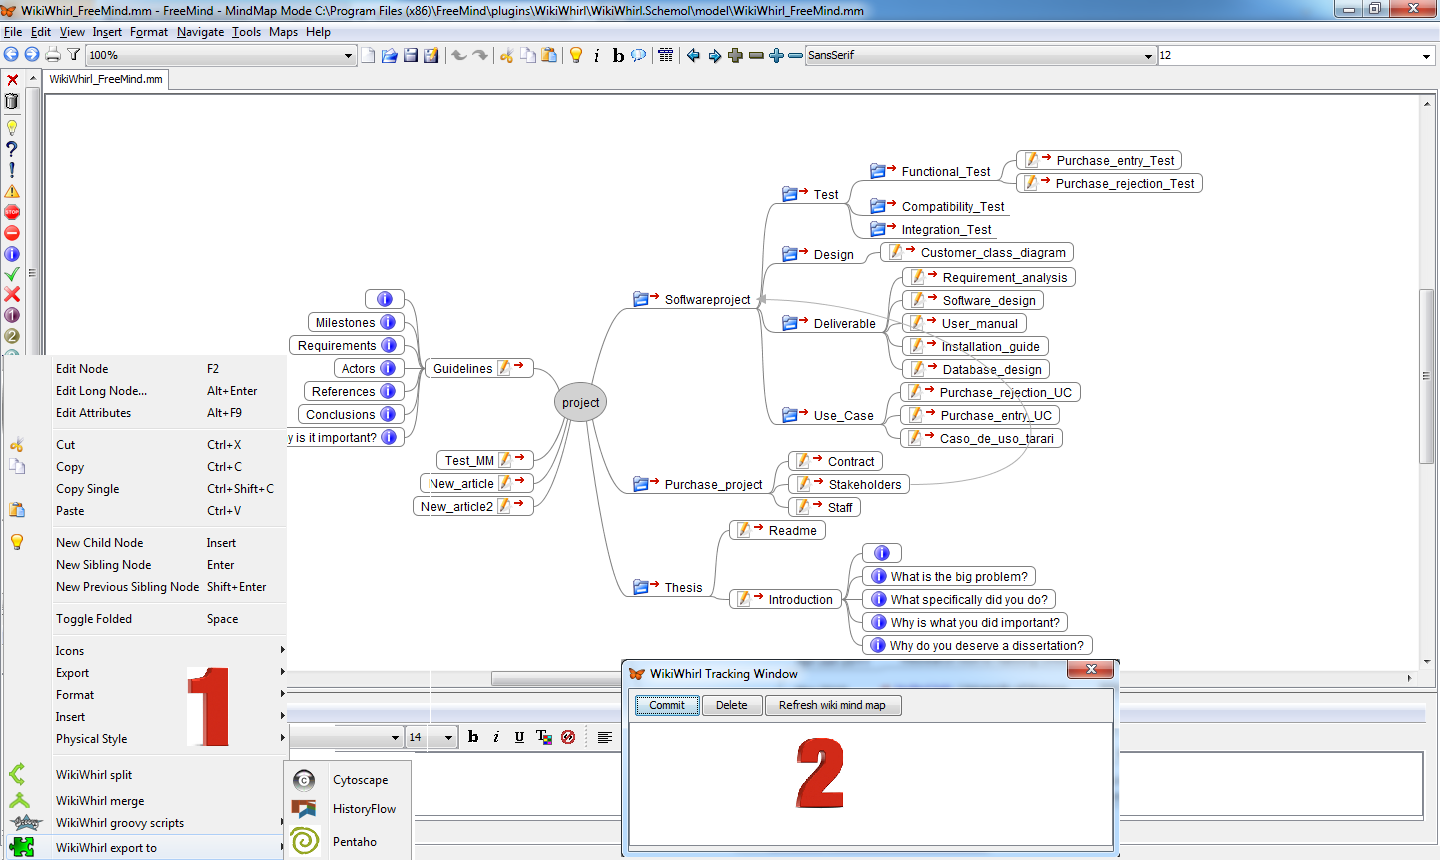
\includegraphics[scale=.4]{images/wikiwhirl_mindmap.png}
	\end{center}
	\caption{A screen shot of WikiWhirl taken from \url{http://www.onekin.org/portal/wikiwhirl}}
\end{figure}

Readership independence is maintained during an article split by adding a summary section where the content that was added to the new article was originally. This allows people reading the source article to still understand what the split of section contained. This process is tedious and poorly supported by the wiki engine which makes it an ideal target for automated refactoring.

WikiWhirl is a visual DSL for refactoring wikis~\citep{wikiMaps}. WikiWhirl is built on top of FreeMind an open source mind mapping tool.\footnote{\url{http://freemind.sourceforge.net/wiki/index.php/Main_Page}} Mind mapping is a method of visualizing the relationships between pieces of  hierarchical information. WikiWhirl represents a wiki as a mind map and users can then refactor the wiki using this view (see figure~\ref{wikiwhirl}). 


WikiWhirl currently supports eight refactorings. They are:

\begin{itemize}
	\item Create an article/category
	\item Categorize an article
	\item Uncategorize an article
	\item Rename an article/category
	\item Delete an article/category
	\item Merge two articles/categories
	\item Split an article/category
	\item Move a section from one article to another
\end{itemize}

Both wikis and spreadsheets are common data formats that deal with the same "smell" and quality issues that software projects experience. The difference between software development and these applications is that the users of the latter will not necessarily be technology professionals. Refactoring tools for wikis and spreadsheets have to be usable by laypeople not just software engineers. 

\section{Refactoring to introduce parallelism}\label{refacParallel}

The reasons to refactor source code have also expanded beyond code quality. This section will describe two different projects that have developed refactorings to change the execution of a program from single to multi-threaded. Functional programming languages are well suited to parallel execution due to immutability by default and in some languages (such as Erlang) first class concurrency features. This section will first describe ParaForming which uses refactoring to introduce parallel abstractions into Haskell code, then it will describe work done to refactor Erlang code to introduce algorithmic skeletons.

\subsection{ParaForming}  
ParaForming is an approach to construct parallel programs from an existing program using software refactoring~\citep{paraforming}. The ParaForming work targets Glasgow parallel Haskell (GpH) an extension to Haskell and is implemented in HaRe. Parallelism is added to programs in GpH using strategies (see figure~\ref{strategy}). 

\begin{figure}[t]\label{strategy}
\begin{lstlisting}
type Strategy a = a -> Eval a
\end{lstlisting}
\caption{The strategy type}
\end{figure}   

A strategy takes its argument and determines how it will be evaluated inside of the \texttt{Eval} monad. The \texttt{rpar} strategy introduces parallelism by "sparking" its argument. A spark allows for something to be evaluated in parallel. However, a spark will only be evaluated in a separate thread if a processor is available, this means that many sparks can be created without adding an unnecessary amount of overhead that actually reduces the programs performance.

The simplest parallel refactoring is introducing data parallelism. This refactoring is applied to an expression that is of type list and evaluates each member of that list in a spark. A sequential function that sums the Euler totient function is in figure~\ref{eulerSeq} and the refactored program is in figure~\ref{eulerPar1}

\begin{figure}[t]\label{eulerSeq}
\begin{lstlisting}
sumEulerSeq :: Int -> Int
sumEulerSeq n = sum (map euler (mkList n))
\end{lstlisting}
\caption{A sequential calculation that sums the Euler totient function}
\end{figure} 


\begin{figure}[t]\label{eulerPar1}
\begin{lstlisting}
sumEulerPar1 :: Int -> Int
sumEulerPar1 n = sum (map euler (mkList n) `using` parList rdeepseq)
\end{lstlisting}
\caption{A refactored version of the function from figure~\ref{eulerSeq}}
\end{figure} 
  
This refactoring evaluates the calculation of \texttt{map euler (mkList n)} using\footnote{The (\texttt{using :: a -> Strategy a -> a}) function just evaluates some value with the given strategy.} the \texttt{parList rdeepseq} strategy. The (\texttt{parlist :: Strategy a -> Strategy [a]}) function evaluates each element of a list in parallel according to a given strategy and \texttt{rdeepseq} is the strategy the fully evaluates its argument. 
  
The refactored program in figure~\ref{eulerPar1} is highly parallel but not very efficient because the parallelism is very fine grained. Another refactoring can help in this case instead of sparking every element of a list another strategy can be introduced, one that separates the list into "chunks" and each of the chunks of the list is executed in parallel. This refactoring adds an additional argument to the function that determines how many chunks the list will be split into, as seen in figure~\ref{eulerChunk}.
  
\begin{figure}[t]\label{eulerChunk}
\begin{lstlisting}
sumEulerChunk :: Int -> Int -> Int
sumEulerChunk c n = sum (map euler (mkList n) `using` parListChunk c rdeepseq)
\end{lstlisting}
\caption{A "chunked" version of the function from figure~\ref{eulerSeq}}
\end{figure}  

These two refactorings are both a way of introducing data parallelism with varying degrees of granularity. The other form of parallelism is known as task parallelism. Task parallelism distributes the calculation of a program across multiple processors, compare this to the data parallelism in figures~\ref{eulerPar1} and \ref{eulerChunk} where the data from the list is distributed across processors instead. 

A divide and conquer version of the \texttt{sumEuler} function is defined in figure~\ref{dncEuler}. The refactoring works by executing the recursive calls on the left and right hand sides of the list in parallel. 

\begin{figure}[t]\label{dncEuler}
\begin{lstlisting}
sumEulerDnc :: [Int] -> Int
sumEulerDnc [] = 0
sumEulerDnc [x] = euler x
sumEulerDnc xd = s1+s2
	where (left, right) = splitAt (length xs `div` 2) xs
				s1 = sumEulerDnc left
				s2 = sumEulerDnc right
\end{lstlisting}
\caption{A divide and conquer version of \texttt{sumEuler}}
\end{figure}

The refactoring targets the \texttt{s1} task from figure~\ref{dncEuler}. An \texttt{Eval} monad is added inside of a let binding in the right hand side of the function definition. Inside this monad the target task is executed in parallel and the calculated value is returned and bound using the let. All occurrences of the task in the original right hand side are then replaced with the let variable. The final result of this refactoring is in figure~\ref{dncPar}. The refactoring leaves the base cases unmodified and so they have been left out of this figure.

\begin{figure}[t]\label{dncPar}
\begin{lstlisting}
sumEulerDnc :: [Int] -> Int
...
sumEulerDnc xd = 
	let s1_2 = runEval $ do
		s1_2 <- rpar s1
		return (s1_2)
	in s1_2 + s2
	where (left, right) = splitAt (length xs `div` 2) xs
				s1 = sumEulerDnc left
				s2 = sumEulerDnc right
\end{lstlisting}
\caption{A task parallel version of the divide and conquer \texttt{sumEuler}.}
\end{figure}

Much like the first version of the data parallel program, the function in figure~\ref{dncPar} has a very fine grained parallelism strategy. The work in~\citep{paraforming} provides a similar refactoring that limits the number of sparks produced.

The goal of this work is to assist programmers in introducing parallelism into their programs and then tuning the level of parallelism to be appropriate to that program.  

\subsection{Cost-Directed Parallel Refactoring}

The previous section touched one of the big challenges of parallel programming, determining the correct level of parallelism to achieve maximum performance. \citep{parallelErl} describes a methodology to introduce algorithmic skeletons into Erlang programs using the Erlang refactoring tool Wrangler. In addition to introducing a skeleton this work provides cost models that estimate the performance of the program after adding each skeleton. This estimate helps a programmer make an informed decision about what parallelisation strategy is the best for a particular program. 

An algorithmic skeleton is a common parallel pattern. A skeleton is implemented as a higher order function that takes in a sequential function and any parameters that the skeleton requires. \citep{parallelErl} discusses the four most common and useful skeletons.

\begin{itemize}
\item \texttt{seq} is the base case skeleton. This skeleton does not introduce any parallelism to the program. 
\item \texttt{pipe} models a pipeline of functions where each functions input is the previous functions output. Parallelisation is gained from executing multiple inputs to the pipeline simultaneously. While one input is passed to a function further down the pipeline the function that just finished can start executing another input.
\item \texttt{farm} applies a single function to a sequence of independent inputs in parallel.
\item \texttt{map} is similar to \texttt{farm}. Each of the inputs to \texttt{map} can be partitioned into a sequence and a worker function can be applied in parallel to each sequence. Finally the results from the worker processes are combined into a single result for each input.   
\end{itemize}

Skeletons are simple to understand in theory but it can be difficult to know which to apply in practice. This is when the cost models of each skeleton become useful to help make an informed decision about which skeleton should cause the greatest speed up. One of the examples presented in~\citep{parallelErl} is that of an image processing system that denoises images. This system is composed of two steps, first geo-referencing information for each image is consolidated then the image is filtered which performs the actual denoising. A simple sequential pipeline of the denoising is defined in figure~\ref{seqDenoise}.

\begin{figure}[t]\label{seqDenoise}
\begin{lstlisting}
denoise(Ims) -> [filter(geoRef(Im)) || Im <- Ims].
\end{lstlisting}
\caption{A sequential denoiser}
\end{figure}    

Obviously cost estimates aren't very helpful without a baseline to compare it to. The timings done in~\citep{parallelErl} show that the geo-referencing stage takes 171 ms and the filter takes 466 ms to process a single image. The complete denoiser computation is just the composition of these two stages so the total cost of processing a single image is the sum of these two costs (637 ms), and the entire system runs over $n$ images in $637*n$ ms. With this baseline established we can compare this to the cost model of refactoring the denoiser parallel pipeline instead. The cost of a pipeline is the the runtime of the costliest step, in this case $(Max(171,466)*n$ which is an improvement over the sequential version of the denoiser. The authors of~\citep{parallelErl} provide a skeleton library in Erlang called \texttt{skel}. The refactorer can be used to transform the denoiser into parallel pipeline as seen in figure~\ref{pipeDenoise}

\begin{figure}[t]\label{pipeDenoise}
\begin{lstlisting}
denoise(Ims) -> skel:run([{pipe, 
	[{seq, fun ?MODULE:geoRef/1}, 
	 {seq, fun ?MODULE:filter/1}]}], Ims).
\end{lstlisting}
\caption{The denoiser as a parallel pipeline}
\end{figure}

Each of the pure functions from the original denoiser are wrapped with the \texttt{seq} skeleton so that they can become steps of the parallel pipeline. The parallelisation of this program doesn't need to stop here. Each of the steps in the pipeline can undergo further refactoring. The filter step for example can be improved using a parallel map. The \texttt{filter} function currently works over the entire image but the filter could be rewritten so that the image was broken up into pieces, those pieces can be filtered in parallel and then another function combines these pieces back together again. The geo-referencing function can't be partitioned in the way that the filter function can but a \texttt{farm} could be introduced so that multiple images can have their geo-references consolidated simultaneously. The final refactored denoise function from~\citep{parallelErl} is defined in figure~\ref{denoiseFinal}.\footnote{The \texttt{Nw} variable passed to the \texttt{farm} determines how many instances of the \texttt{geoRef} function will be sparked.}


\begin{figure}[t]\label{denoiseFinal}
\begin{lstlisting}
denoise(Ims) -> skel:run([{pipe, 
	[{farm, [{seq, fun ?MODULE:geoRef/1}], Nw}, 
	 {parmap, [{seq, fun ?MODULE:filter/1}],
		fun ?MODULE:partition/1,
		fun ?MODULE:combine/1	 
	 }]}], Ims).
\end{lstlisting}
\caption{The denoiser as a pipeline of a farm and a parallel map.}
\end{figure}

Parallelisation can be tedious and difficult to do which makes it a good candidate for tool assistance. The refactoring tool can guide a programmer though the process of parallelisation. Much like the how data-driven refactorings have multiple small changes are required before the entire process can be considered "finished" changing a program to run in parallel is also a sequence of many smaller changes.

\section{ApplicativeDo}

\comment{This is just taken from the IFL paper directly}

The under-utilisation of applicatives in Haskell has not gone un-noticed; \citep{applicativeDo}, reimplement the way Haskell desugars do notation so that applicatives will be supported by do notation as well. 

\begin{lstlisting}
f = do
	x1 <- A
	x2 <- B x1
	x3 <- C
	return (x2,x3)
\end{lstlisting}

The function \texttt{f} would normally desugar into the following:

\begin{lstlisting}
f = A >>=
	(\x1 -> B x1 >>=
		(\x2 -> C >>=
			(\x3 -> return (x2,x3))))
\end{lstlisting}

With applicative do activated \texttt{f} would now desugar to:

\begin{lstlisting}
f = (\x2 x3 -> (x2, x3))
        <$> (A >>= (\x1 -> B x1))
        <*> C                
\end{lstlisting}

The \texttt{ApplicativeDo} algorithm will attempt to insert as many applies into the expression as possible. When the implementation of the \texttt{Applicative} instance evaluates the two arguments of apply in parallel, better performance can be achieved by adding more applies. 

There could be multiple ways to desugar a particular function. The \textit{applicativeDo} algorithm first assumes that every expression have an identical time cost, from this assumption the algorithm heuristically determines the desugaring with the shortest execution time.


\section{Program transformations}\label{typeTrans}

Refactoring is a type of program transformation but it does not constitute the whole field. A major difference between refactoring and other types of program transformations is the interactivity that a refactoring must support. A refactoring needs to be well understandable by programmers because must choose to apply a refactoring manually and using the refactoring tool needs to be easier than performing the transformation manually. Additionally the target program of a refactoring needs to be readable, maintainable, and keep proper layout and user comments. Other types of program transformation don't typically have these concerns. This section will describe some of the program transformation work most relevant to this thesis. First it will describe the type and transform system developed by~\citep{typeAndTransformSemantics}. Next there will be a discussion of the previous methods of monadification found in the literature. 

\subsection{Type and transform systems}

The type-and-transform system described in~\citep{typeAndTransformSemantics} is a system for a semantics preserving and type changing program transformations over the typed lambda calculus with let polymorphism. The type-and-transform system is limited to isomorphic types, there must be a way to convert between the two types and back again as described in figure~\ref{transformIso}.

\begin{figure}[t]\label{transformIso}
\begin{lstlisting}
rep :: A -> R
abs :: R -> A

rep . abs = id
abs . rep = id
\end{lstlisting}
\caption{The properties that must hold for the type-and-transform system to work over types \texttt{A} and \texttt{R}}
\end{figure} 

The type-and-transform system supports type-changing rewrites through typed rewrite rules 
\comment{I'm really at a loss for how this system works and how to describe it.}

\subsection{Automatic Monadification}\label{erwigMonad}

Monadification is not a new problem and various solutions have been presented in the literature. In~\citep{lammelReuse} monadification is performed in two steps. First the program is transformed into A-normal form\footnote{This is also known as sequencing}, which flattens applications into let expressions. The first line of figure~\ref{anormal} shows a normal expression and line 3 of the same figure shows that expression in A-normal form.

\begin{figure}[t]\label{anormal}
\begin{lstlisting}
f (g x) (h y)

let x1 = g x in
	let x2 = h y in
		f x1 x2
\end{lstlisting}
\caption{A-normal form converstion}
\end{figure}

Once the program has been converted into A-normal a let expression of the form $ let x = t1 in t2 $ is transformed into $ t1 >>= \lambda x. t2 $. If the right hand side of the lambda isn't already a monadic type then \texttt{return} will be introduced, e.g. $ t1 >>= \lambda x. return~~t2 $. The full transformation is given by inference rules in~\citep{lammelReuse}.

Monadification is developed further by~\citep{monadification}. This work provides an algorithm for monadification as opposed to the semantics style inference rules defined in~\citep{lammelReuse}. \citep{monadification} also 

\subsubsection{Issues with Erwig and Ran's solution}

There are a few issue with the monadification solution proposed by~\citep{monadification}. There several different styles of monadification and this algorithm only supports one of them~\citep{clausMonadResponse}. Five different styles of monadification have been outlined in~\citep{monadSurvey}, and before implementing an automatic monadification solution it should be determined which style of monadification would be the most helpful to the Haskell community.

\chapter{Conclusion}
Summarise my contribution here. The main contributions of my thesis are the development of type changing refactorings for GHC. With a particular emphasis on changing the abstractions that programs use.

\bibliography{main}

% This index section is optional, use cleardoublepage and phantomsection to make the links work in your contents page. Uses makeidx package.
\cleardoublepage
\phantomsection
\label{index}
\printindex

\end{document}
